\documentclass{ATLAS_latex/atlasnote} 
\skipbeforetitle{-5pt}

\usepackage{graphicx,multirow}
\usepackage{epstopdf}
\usepackage{authblk}
\usepackage{hyperref}
\usepackage{pdfpages,subfigure,caption,placeins}
\usepackage{color}

\newcommand{\red}[1]{\textcolor[rgb]{1,0,0}{#1}}

\input{tex/definitions}
\input{tex/prd_definitions}

\renewcommand{\topfraction}{0.95}
\renewcommand{\bottomfraction}{0.8}
\renewcommand{\textfraction}{0.06}
\renewcommand{\floatpagefraction}{0.85}
\setcounter{totalnumber}{5}
\setcounter{topnumber}{4}

\bibliographystyle{apsrev}

\title { Diamond-paved roads and a steaming soup: the architecture of an upgraded Micromegas trigger processor and an optimization tool}
%that 
%mitigates the degradation of the {\boldmath $\eta$} and {\boldmath $\phi$} resolutions
%caused by the expected background rates}

\usepackage{authblk}
\renewcommand\Authands{, } % avoid ``. and'' for last author
\renewcommand\Affilfont{\itshape\small} % affiliation formatting
\author[a]{N.~Felt}
\author[a]{M.~Franklin}
\author[a]{P.~Giromini}
\author[a]{A.~Tuna}
\author[a]{A.~Wang}
\affil[a]{Harvard University, Cambridge, Massachusetts 02138, USA}
\affil[b]{University of Massachusetts Boston, Boston, Massachusetts 02125, USA}

\abstracttext{\noindent We have developed a simple simulation tool, HOTPOT, to investigate the performance of
 the Micromegas trigger processor (MMTP) in the presence of the uncorrelated-background rate expected at the high-luminosity LHC.
  The study was motivated by our measurement of the MMTP  spatial resolution using the Harvard octuplet and cosmic rays.
 Having  observed that the MMTP  architecture outlined in the NSW TDR already loses efficiency and spatial resolution because of the irreducible background due to $\delta$ rays, we  simulate the effect of the expected uncorrelated background overlapping muon signals, and find
  that the performance of the planned MMTP scheme is severely degraded. Therefore, we propose a new architecture which is less affected by the presence of this background and present its expected performance. }

\clearpage

\begin{document} 

\setcounter{page}{2}

\section{Introduction}
\label{sec:intro}

The previous note \cite{mmtp} reported that based on the measured ART resolution, the MMTP algorithm requires an ART collection window of 6-8 BCs for a fully efficient trigger. Furthermore, we saw that the MMTP performance was extremely sensitive to correlated background hits from $\delta$-rays. To study the effect of uncorrelated background, we implement a faithful software simulation of the MMTP algorithm, called the Harvard Octuplet Trigger Performance Optimization Tool (HOTPOT). 


%\input{tex/experiment}
\section{High luminosity LHC}
\label{sec:hllhc}

Over the next twenty years, the LHC plans to steadily increase the rate at which proton-proton collisions are delivered to the ATLAS and CMS experiments. The final design of the machine, called the High Luminosity LHC, could potentially deliver a peak instantaneously luminosity of $\mathcal{L} = 7.5\times10^{34}\text{ Hz/cm}^2$. This is almost ten times larger than the original design luminosity of the LHC of $\mathcal{L} = 1\times10^{34}\text{ Hz/cm}^2$~\cite{lhc}. It is clear that the predicted instantaneously luminosity is an estimate, and experiments would be prudent to consider the effect of even higher luminosity.

To predict the hit rate in the NSW at the HL-LHC, the hit rate in the current Small Wheel is measured and extrapolated to higher luminosity~\cite{tuna,phase2}. The measured hit rate increases linearly with the luminosity, as expected, giving confidence to the extrapolation. The current SW is comprised of MDT and CSC detectors, and detector effects are factored out to give a detector-independent prediction for the NSW.

The prediction is shown in Fig.~\ref{fig:rate_vs_r} as a function of $R$, the radial distance from the beamline. On the left is the predicted rate per unit area, and on the right is the predicted rate per Micromegas strip. For simplicity, some results in this note are presented with an uncorrelated background rate of 40 kHz per strip, which corresponds to the rate prediction near the beamline. For prudence, other results are presented as a function of the hit rate.
\begin{figure}[!htpb]
  \begin{center}
    \includegraphics[width=0.48\textwidth]{figures/ilia.pdf}
    \includegraphics[width=0.48\textwidth]{figures/rate_per_strip.pdf}
  \end{center}
  \vspace{-10pt}
  \caption{Predicted rate vs. distance from the beamline at $\mathcal{L} = 7.5\times10^{34}\text{ Hz/cm}^2$, per unit area (left) and per strip (right). The rate per area is culled from the Phase 2 Muon TDR~\cite{phase2}. The rate per strip is derived from the rate per area and the expected area of the Micromegas chambers.}
  \label{fig:rate_vs_r}
\end{figure}


\section{Simulation}
\label{sec:sim}

To investigate the performance of the trigger under HL-LHC conditions, we developed HOTPOT, a standalone simulation of the MMTP trigger in C++. We simulate downward moving cosmic tracks, with a variable rate of background, in a rectangular region of the MM detector. We look at two lengths of strips: 2.2 m and 0.5 m, which should capture the trigger performance at the top of LM2 and the bottom of SM1. The output of the simulation is a collection of possible triggers found by the MMTP. For each event, we generate one downward muon track, and then add background hits in a window 40 BCs wide, where the first background hit comes 16 BCs before the first muon hit.
\par We aim to be as faithful and complete as possible. To consider several upstream electronics effects, some of which are not considered in the current ATHENA simulation, we ``feed" the cosmic track hits and background hits through the VMM and the ADDC. This includes the 8-ART signal per BC processing limit of the ADDC and the 1-ART signal per BC limit of the VMM. The position of the cosmic muon hit is also smeared with a gaussian with a $\sigma$ of 1 strip. This is motivated by our previous trigger data, described in \cite{mmtp}. Fig. \ref{fig:art_xres} shows the position resolution of the ART. The RMS of the distribution is about 0.5 mm, or approximately the strip pitch. The timing of the hit is smeared with a gaussian with a $\sigma$ of 32 ns to simulate the ART time resolution measured in \cite{mmtp}.
\begin{figure}[!htpb]
  \begin{center}
    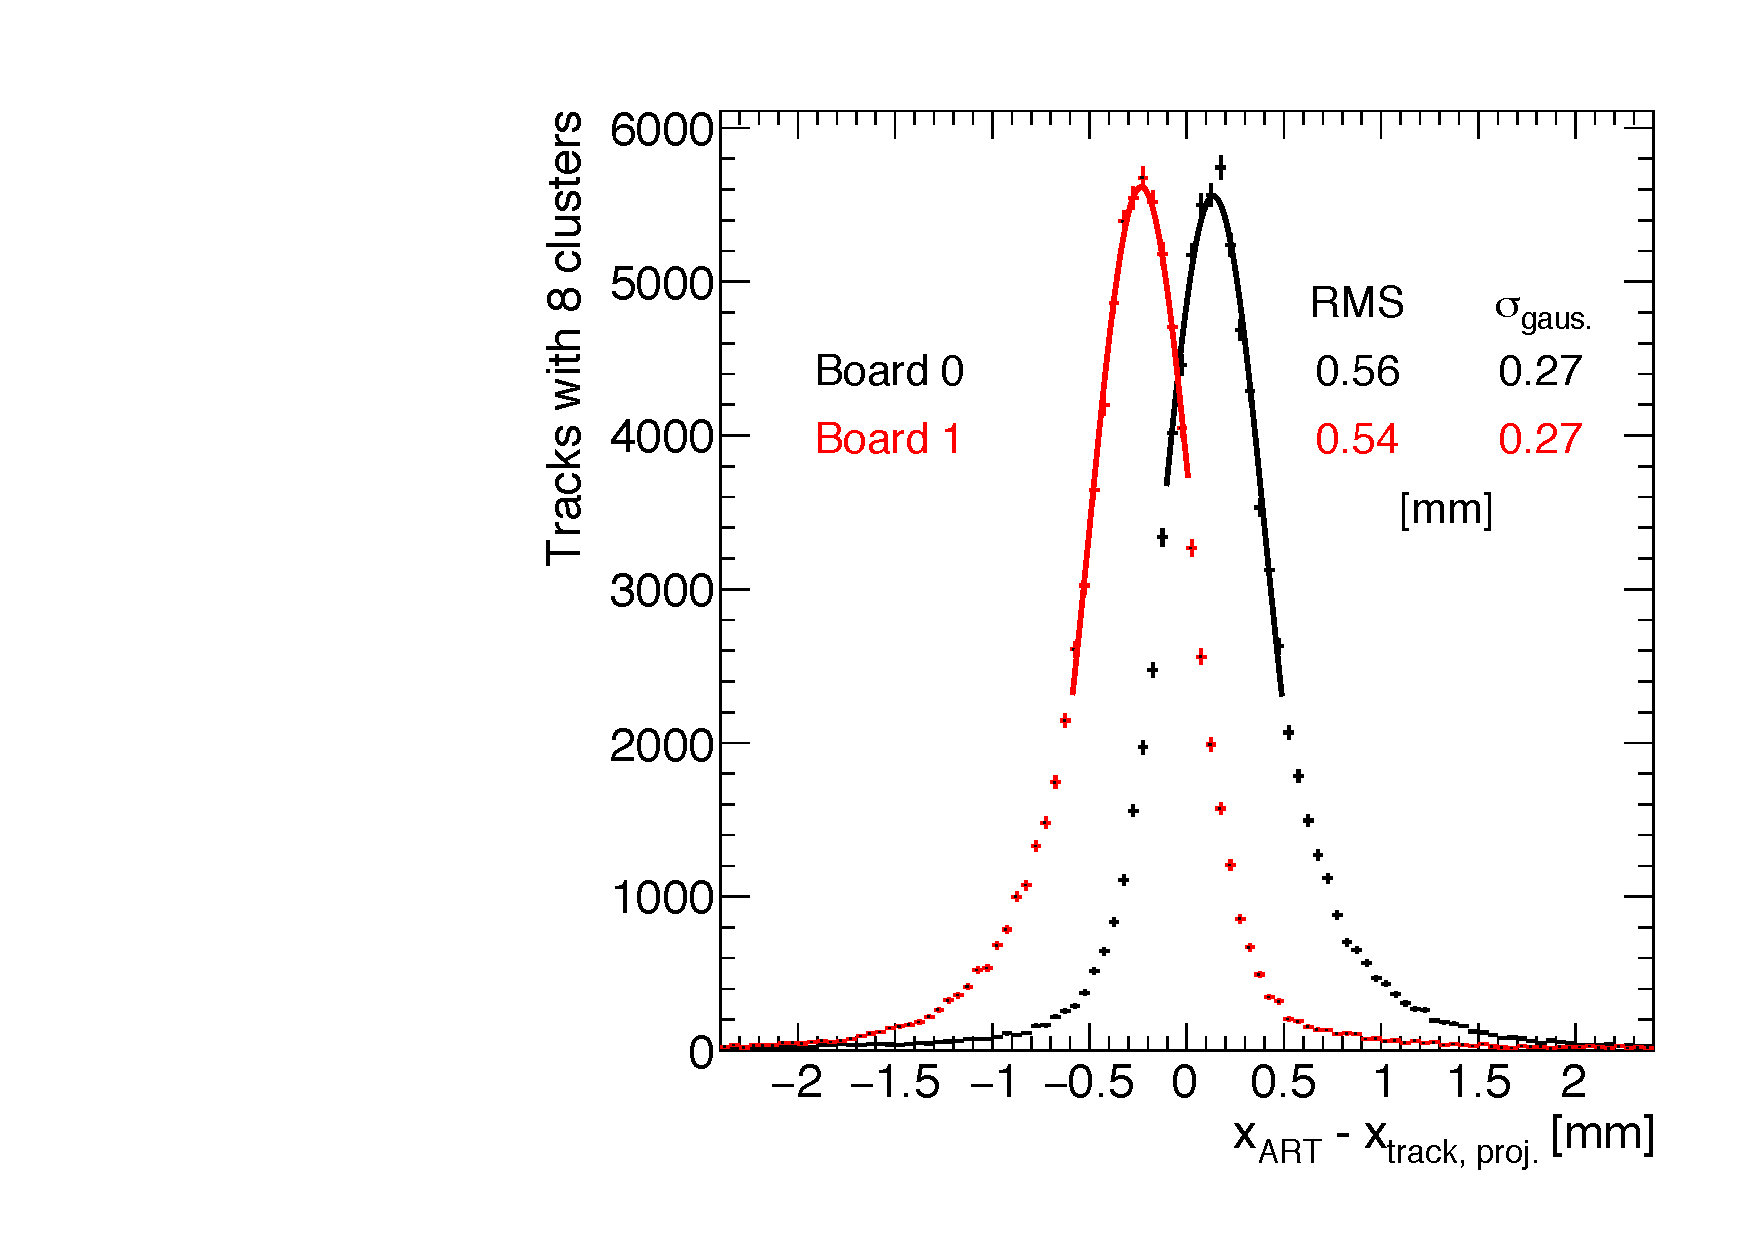
\includegraphics[width=0.48\textwidth]{figures/xres_art_boards01.pdf}
    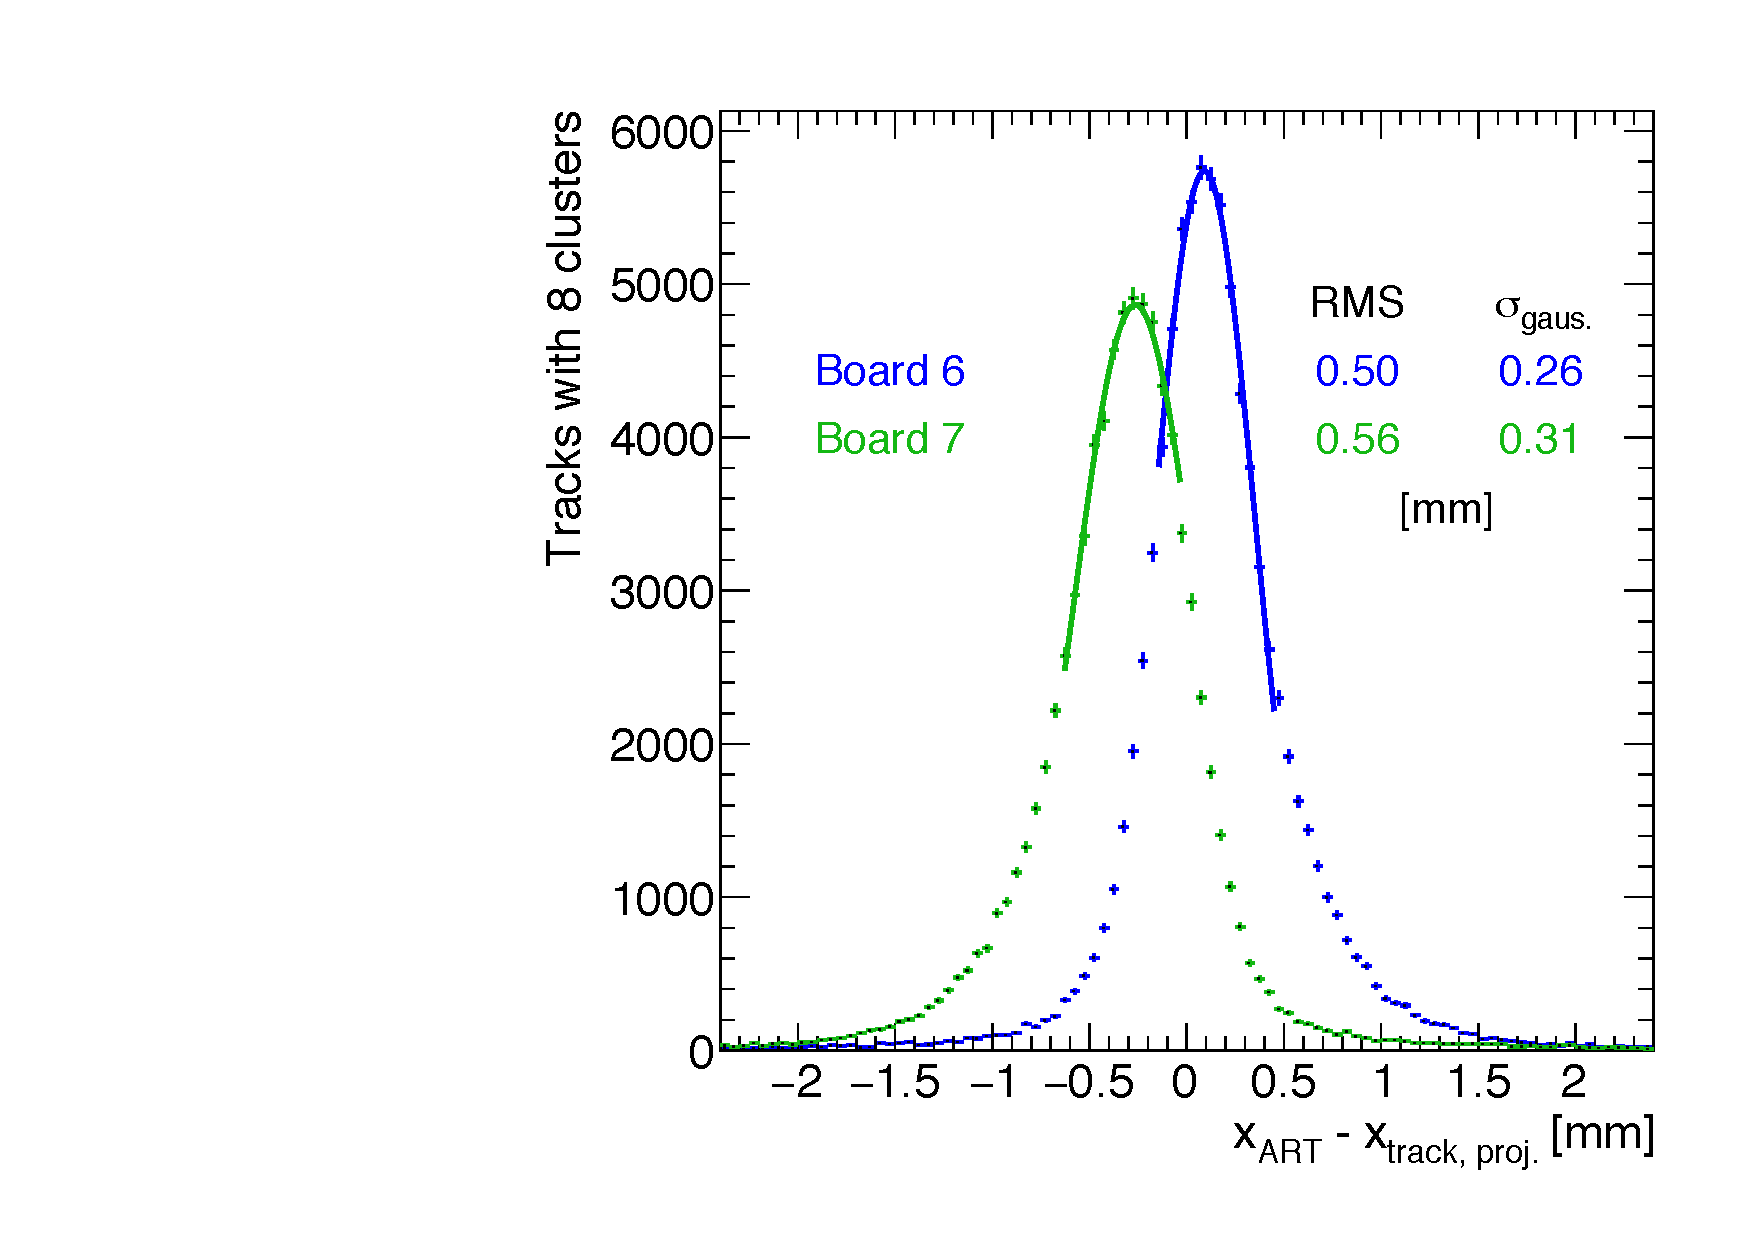
\includegraphics[width=0.48\textwidth]{figures/xres_art_boards67.pdf}
  \end{center}
  \vspace{-10pt}
  \caption{The x-residuals (precision coordinate) of the ART hit compared to the projected x-position using a track fit to 8 MMFE8 clusters, for each of the $X$ boards, indexed 0 \& 1 (left), 6 \& 7 (left).}
  \label{fig:art_xres}
\end{figure}

\par 
We then feed the ART hits through an implementation of the MMTP algorithm. The algorithm has two versions: the nominal (original) algorithm, and the proposed algorithm, described in Sections \ref{sec:nominal} and \ref{sec:stereoroads}, respectively. The algorithm collects ART hits over a fixed time collection window (8 BCs), looks for and then outputs candidate triggers. Since the interface with the sTGC detectors and Sector Logic has yet to be determined, we study the resolution by ordering the output triggers by how many hits they contain from the original muon track (dubbed ``real muon hits"). We then randomly choose one of the triggers with the maximum number of real muon hits.
There are several tunable parameters that are affect the MMTP performance. The list of parameters and their default values are given in the following table:
\begin{center}
\begin{tabular}{ |c|c| } 
 \hline
 \textbf{Parameter} & \textbf{Default Value} \\ 
 MM chamber efficiency & 100\%  \\ 
 ART time resolution (ns) & 32 \\ 
 ART time collection window (BC) & 8 \\ 
 Nominal road size (strips) & 8 \\
 ART position resolution (strips) & 1\\
 Trigger plane coincidence requirement & 3X3UV \\
 Uncorrelated background rate (kHz) per strip & 40\\
 Region size (roads) & 2.2 m strips: 136, 0.5 m strips: 96\\
 \hline
\end{tabular}
\end{center}

\section{Nominal algorithm}
\label{sec:nominal}
\begin{figure}[!htpb]
  \begin{center}
    \includegraphics[width=0.48\textwidth]{figures/cartoon_roads_small_nominal.pdf}
    \includegraphics[width=0.48\textwidth]{figures/cartoon_roads_large_nominal.pdf}
  \end{center}
  \vspace{-10pt}
  \caption{Sketch of the road coverage of the nominal MMTP algorithm, for a small chamber closest to the beamline (left) and large chamber farthest from the beamline (right). The $X$ road is horizontal, the $U$ road is pink and slanted, and the $V$ road is blue and slanted. The x-axis and y-axis are in units of strip pitches, which are set to be 0.4 mm.}
  \label{fig:cartoon_nominal}
\end{figure}
The MMTP algorithm in its current form is described in \cite{mmtp}. We encourage the reader to begin there. In addition, there are a few details which we will elaborate on in this section.
\par As a reminder, the MMTP relies on the concept of roads to form coincidences for a trigger. The wedge is divided into roads which define a set of strips on each plane. The MMTP receives ART hits and places them in the corresponding road. The MMTP looks for a coincidence of a fixed number of planes with hits in a road, within the ART time collection window.
\par Each implementation of the MMTP algorithm covers  a fixed but to-be-determined number of roads. For this study, we will use region sizes of 136 roads and 96 roads for the 2.2 m long strips and 0.5 m long strips, respectively. The motivation for these region sizes is further discussed in Section \ref{sec:stereoroads}. 
\begin{figure}[!htpb]
  \begin{center}
    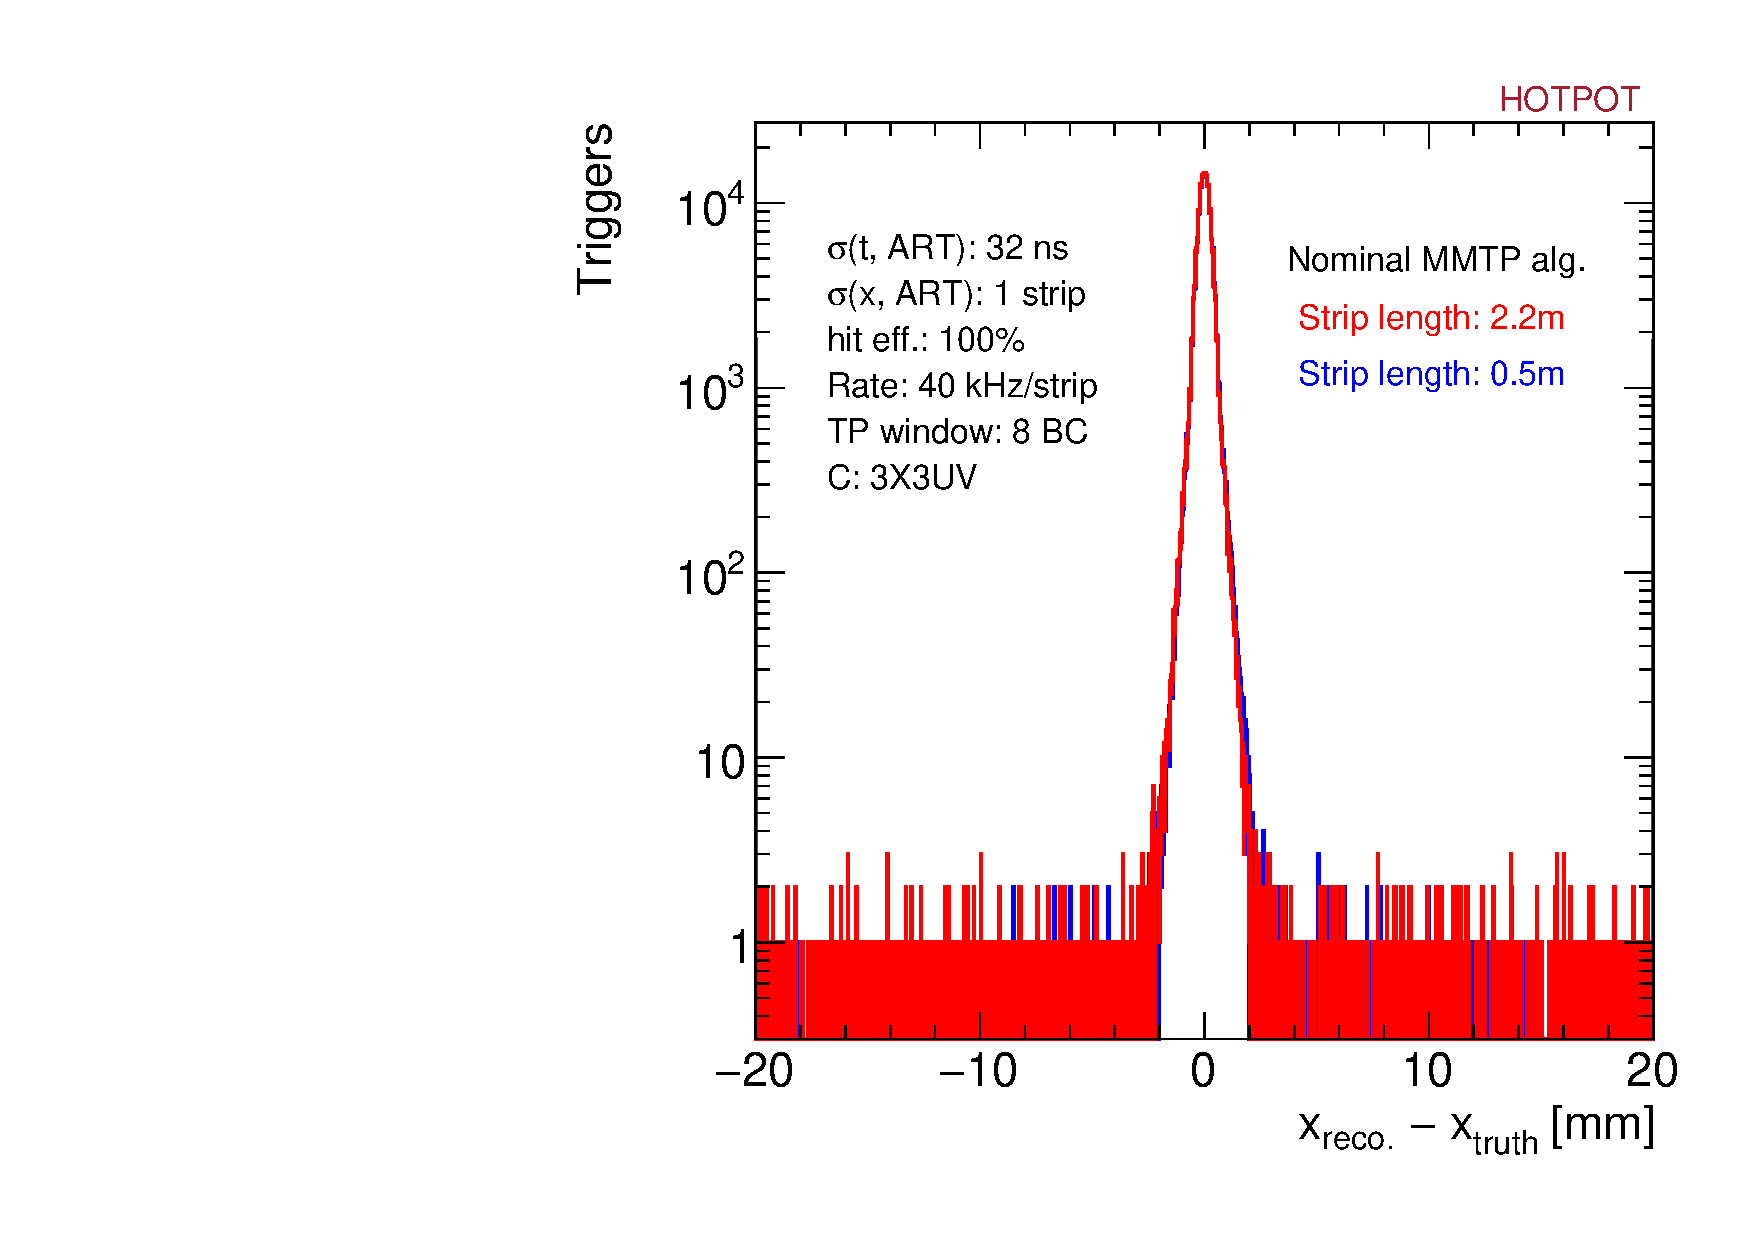
\includegraphics[width=0.48\textwidth]{figures/xres_old.pdf}
    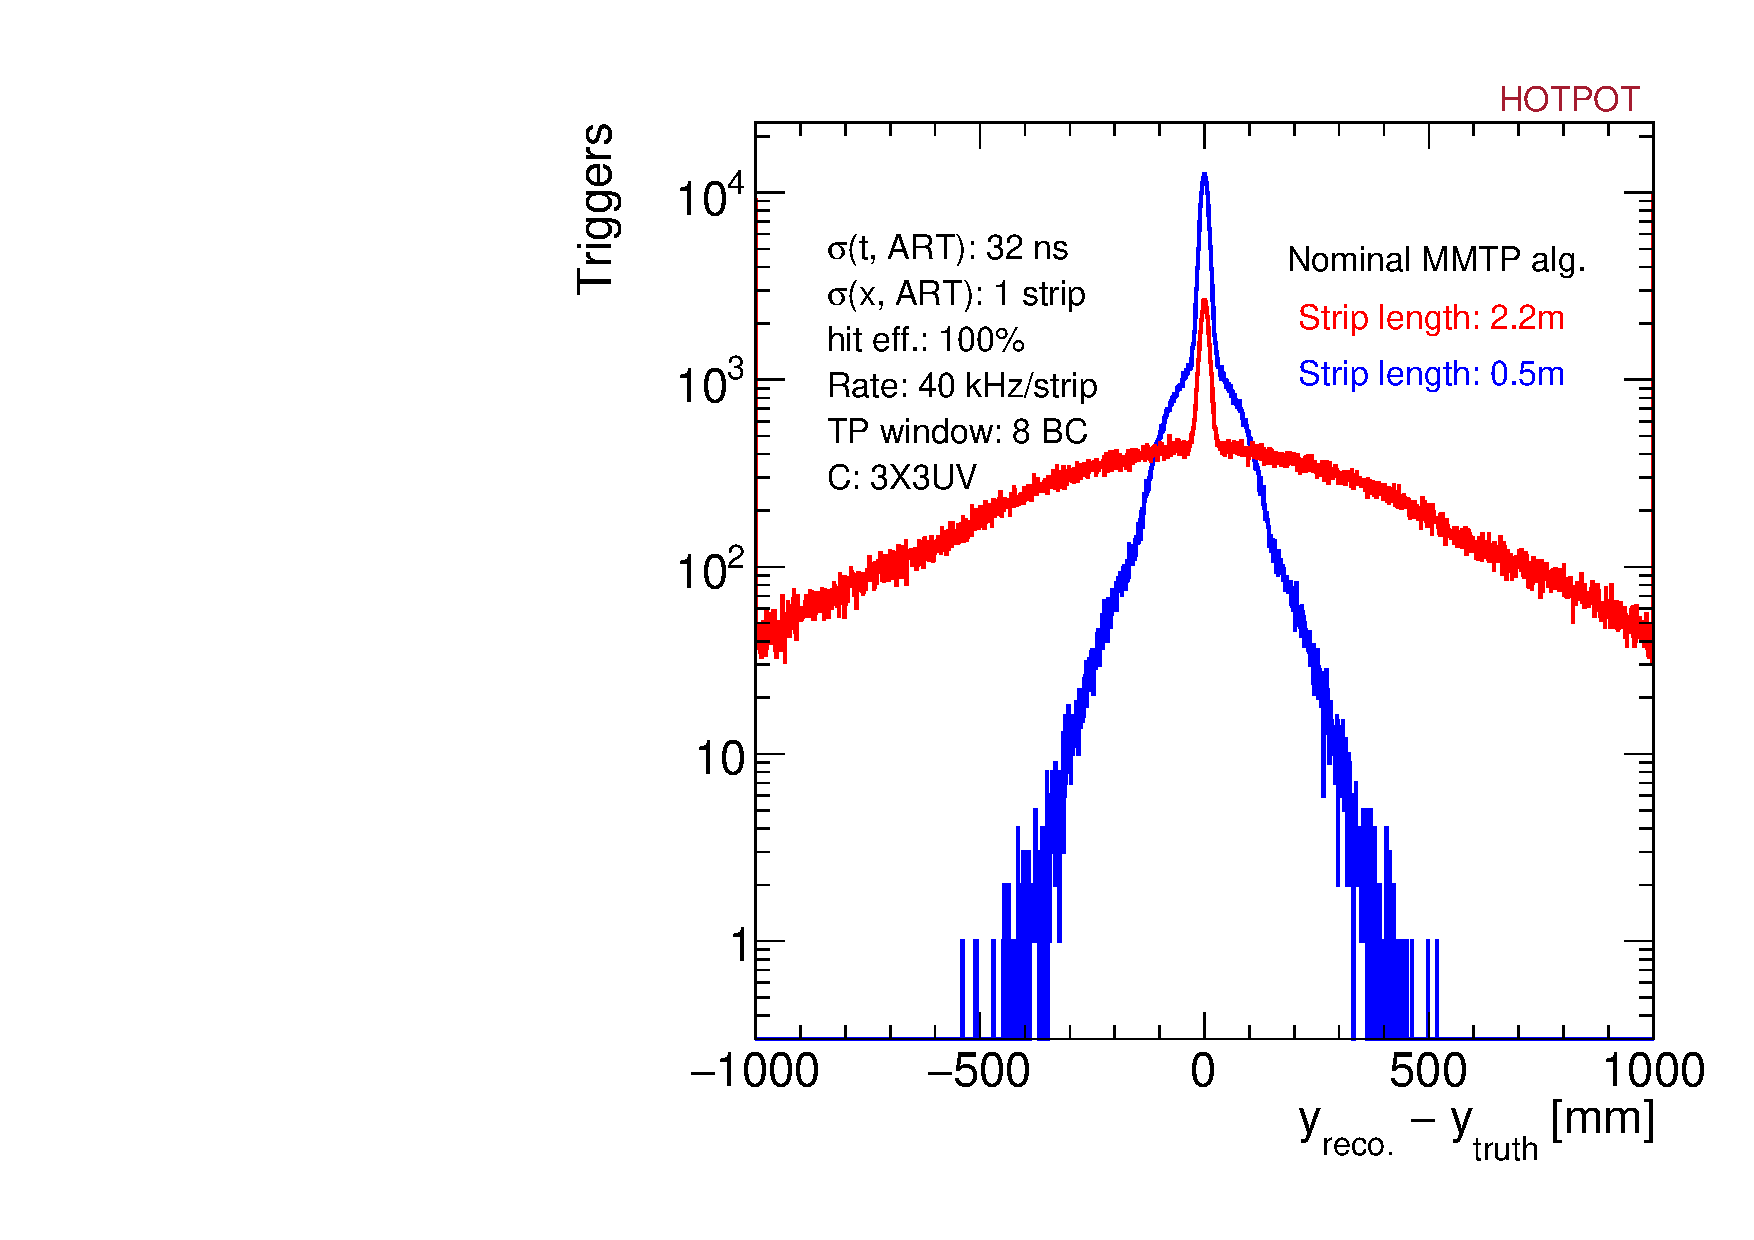
\includegraphics[width=0.48\textwidth]{figures/yres_old.pdf}
    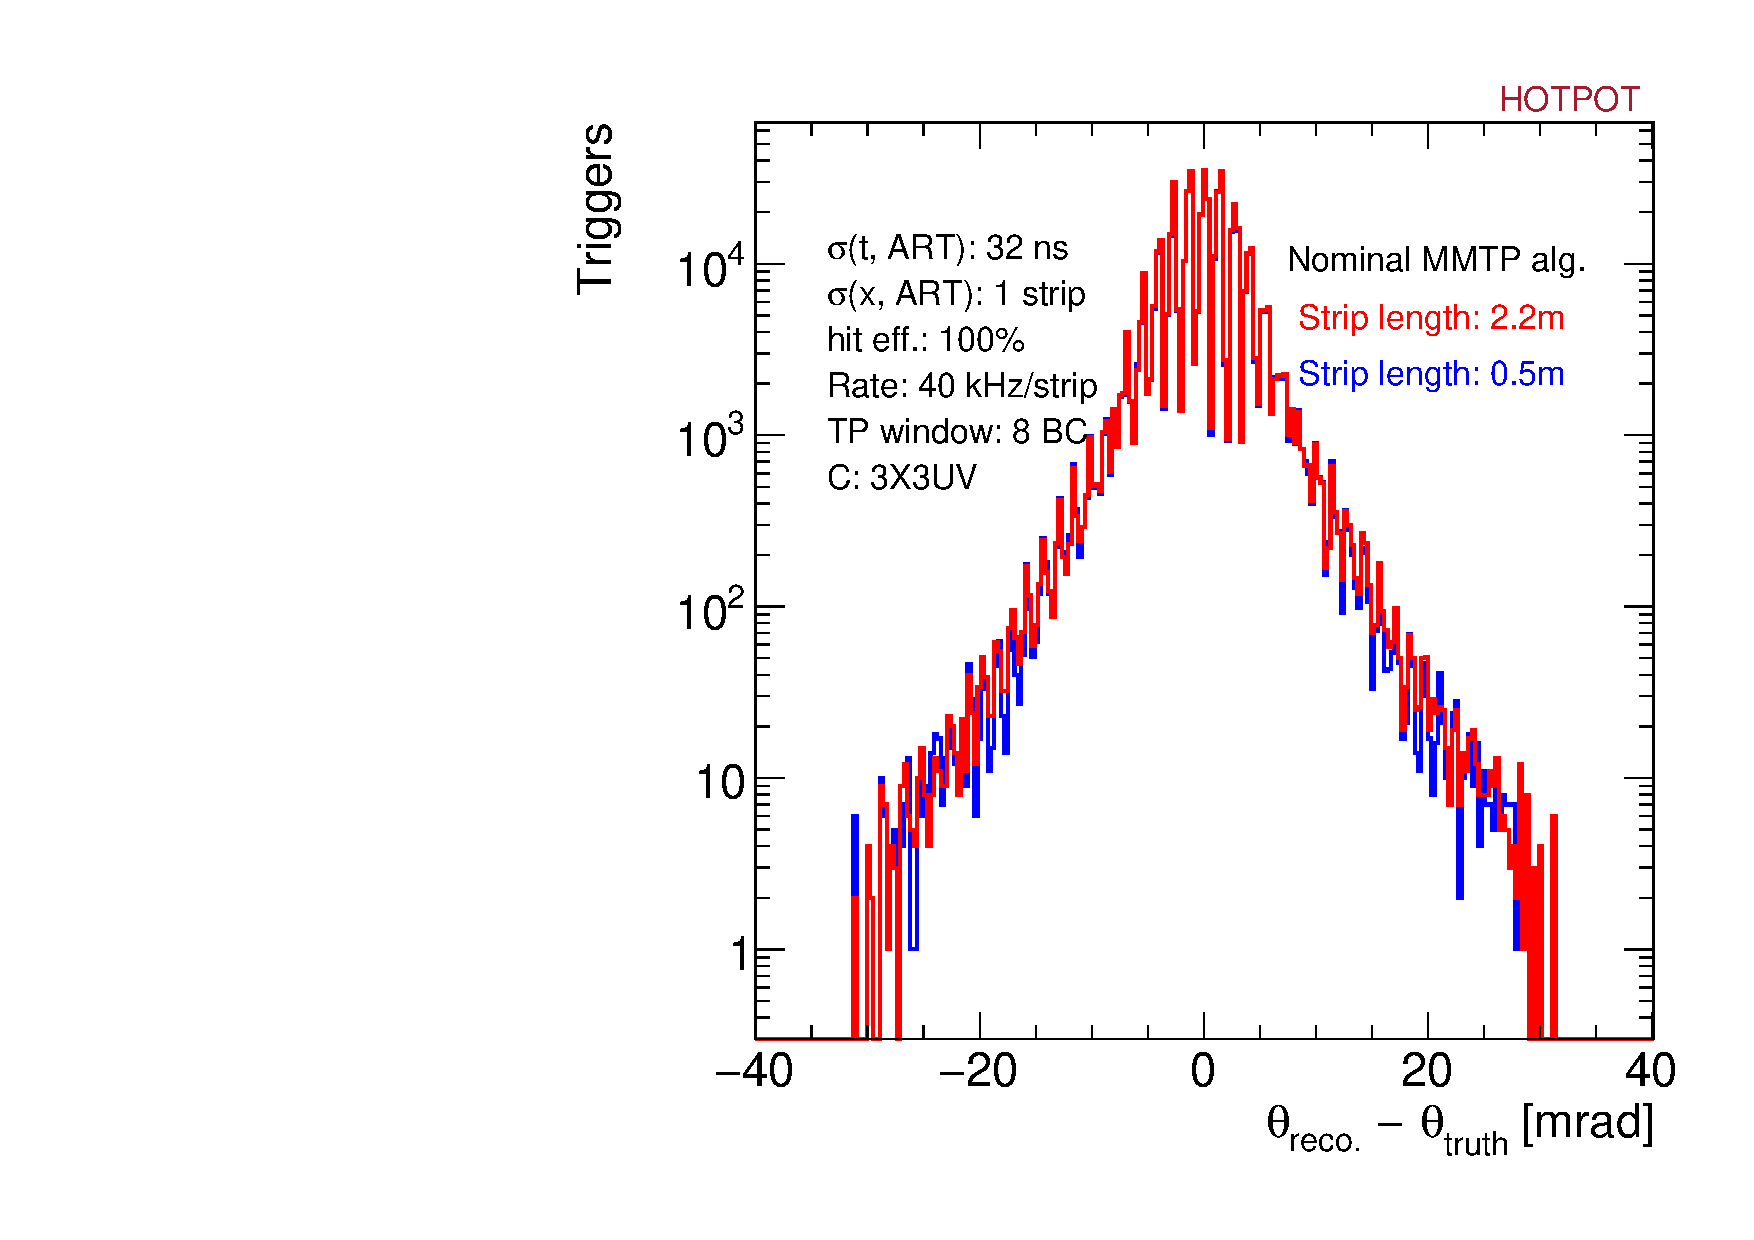
\includegraphics[width=0.48\textwidth]{figures/mres_old.pdf}
  \end{center}
  \vspace{-10pt}
  \caption{Distribution of $x_\text{reco.} - x_\text{truth}$ (top, left), $y_\text{reco.} - y_\text{truth}$ (top, right) and $\theta_\text{reco.} - \theta_\text{truth}$ (bottom) for the nominal MMTP algorithm with uncorrelated background at a rate of 40 kHz per strip.}
  \label{fig:resolutions_old}
\end{figure}
\par Each road spans a certain number of strips on the eight planes in a wedge. The $X$ road size is the number of strips each road spans on on an x plane, and similar definitions apply to the $U$ road size and the $V$ road size. \par To mitigate edge effects when a track spans two roads, each road also sees any hits on ``neighboring" roads (described in more detail in \cite{mmtp}). We note here that we only need to look for hits on one neighboring road to fix these cases, as opposed to both neighboring roads. Furthermore, we modify the scheme so that each road can only see hits on half of the neighboring road. For example, an $X$ road of 8 strips also sees any hits on the adjacent 4 strips. 
\par The $U$,$V$ road size is determined by the $X$ road size. In order for a $U$ or $V$ road to overlap spatially with the entire $X$ road, the $U$,$V$ road size must be larger or equal to the number of strips in an $X$ road plus the number of strips in a neighbor, plus $\tan 1.5^\circ \times \frac{ \text{strip length} }{ \text{strip pitch} }$. Figure \ref{fig:cartoon_nominal} illustrates the effect of the stereo angle on the $U$,$V$ road size.


Figure \ref{fig:resolutions_old} shows the resolution of the MMTP triggers using the nominal algorithm. The reconstructed x position residuals, where x is the precision coordinate, is a narrow distribution bounded by the small $X$ road size, but the reconstructed y resolution is very poor. The RMS calculated in the 3$\sigma$ range of the distribution is 433.4 $\pm$ 0.4 mm for 2.2m long strips. For 0.5m long strips, the 3$\sigma$ RMS is 55.59 $\pm$ 0.05 mm. With a high rate of background, the size of the $U$, $V$ roads makes the trigger extremely vulnerable to background hits. On average, 1.7 stereo plane hits in the track are from background events. In addition, an important consequence of the use of roads in the MMTP algorithm is that each road can only record one ART hit per plane per BC collection window. With large $U$,$V$ roads, a background hit can easily cause the loss of a real muon hit. 

\section{Small stereo roads}
\label{sec:stereoroads}
\begin{figure}[!htpb]
  \begin{center}
    \includegraphics[width=0.48\textwidth]{figures/cartoon_roads_small_smallstereo_1.pdf}
    \includegraphics[width=0.48\textwidth]{figures/cartoon_roads_large_smallstereo_1.pdf}
  \end{center}
  \vspace{-10pt}
  \caption{Sketch of the road coverage of the proposed MMTP algorithm, for a small chamber closest to the beamline (left) and large chamber farthest from the beamline (right). The $X$ road is horizontal, the $U$ road is pink and slanted, and the $V$ road is blue and slanted. For ease of digestion, only one pair of $U$ and $V$ roads are shown, and they do not cover the entire $X$ road. The x-axis and y-axis are in units of strip pitches, which are 0.4 mm.}
  \label{fig:cartoon_smallroads_1}
\end{figure}
\begin{figure}[!htpb]
  \begin{center}
    \includegraphics[width=0.48\textwidth]{figures/cartoon_roads_small_smallstereo_N.pdf}
    \includegraphics[width=0.48\textwidth]{figures/cartoon_roads_large_smallstereo_N.pdf}
  \end{center}
  \vspace{-10pt}
  \caption{Sketch of the road coverage of the proposed MMTP algorithm, for a small chamber closest to the beamline (left) and large chamber farthest from the beamline (right). The $X$ road is horizontal, the $U$ roads are pink and slanted, and the $V$ roads are blue and slanted. The small chamber requires five pairs of $U$ and $V$ roads to cover one $X$ road, and the large chamber requires 19. The x-axis and y-axis are in units of strip pitches, which are 0.4 mm.}
  \label{fig:cartoon_smallroads_N}
\end{figure}
Due to the degraded performance of the nominal algorithm given a high uncorrelated background rate, we propose a modified, improved version of the algorithm.
We can divided each large $U$,$V$ road into multiple roads that are the same size as the $X$ road. Then, each $X$ road has multiple associated $U$,$V$ roads. The overlap of one set of these roads forms a single diamond, which is illustrated in Figure \ref{fig:cartoon_smallroads_1}. To span the length of the chamber, we have a cascade of diamonds, illustrated in Figure \ref{fig:cartoon_smallroads_N}. This dramatically narrows the spatial region in which a coincidence is found. This also reduces the chance that a muon track hit is overwritten by a background hit. Note that it is important that the coincidence threshold be at least 3 X-planes and 3-U,V planes to reduce background triggers. The background rate goes with the $\text{hit rate per plane}^{\text{number of planes}}$.  
\par The performance of the improved algorithm is shown in Figure \ref{fig:resolutions_new}. As expected, the x-resolution is comparable to that of the nominal algorithm, but the y-resolution shows a dramatic improvement. The 3$\sigma$ RMS is 11.29 (12.68) $\pm$ 0.01 (0.01) mm for 0.5m (2.2m) long strips.The y-residual bounds go with the effective $U$,$V$ road size divided by the tangent of the stereo angle. We can also look at the efficiency of a $\Delta \phi <$ 20 mrad cut as a function of the uncorrelated background rate for both algorithms. In Figure \ref{fig:eff_vs_rate}, we see that the performance of the nominal algorithm drops sharply with increased background, while the proposed algorithm maintains 80\% (95\%)+ efficiency for up to a 60 kHz/strip background rate with 0.5m (2.2m) long strips.
\par We now elaborate on the use of implementation regions. It is important to divide the wedge into reasons so that each implementation of the firmware has a minimum number of triggers to process at any given time. There will be hard limit to how many triggers can be processed per BC per implementation. Thus, small implementation regions are ideal. As a technical aside, the exact number of roads in an implementation region is presently determined by the architecture of the MMTP firmware. \footnote{The MMTP relies on multiplexers to select the $U$,$V$ roads overlapping with each $X$ road. If we consider the LM2 with a pitch of 450 microns, we have $2.2\text{m} \times \tan 1.5^\circ \times \frac{1}{450 \;\mu m \times 8 \text{ strips/road}} = 16 + 1$ $U$,$V$ roads associated to one $X$ road, so we need 17 multiplexers. Assuming standard multiplexer of 8:1, we can have 136 $X$ roads in the largest R region. A similar calculation can be done for the 0.5m strips.} 

\begin{figure}[!htpb]
  \begin{center}
    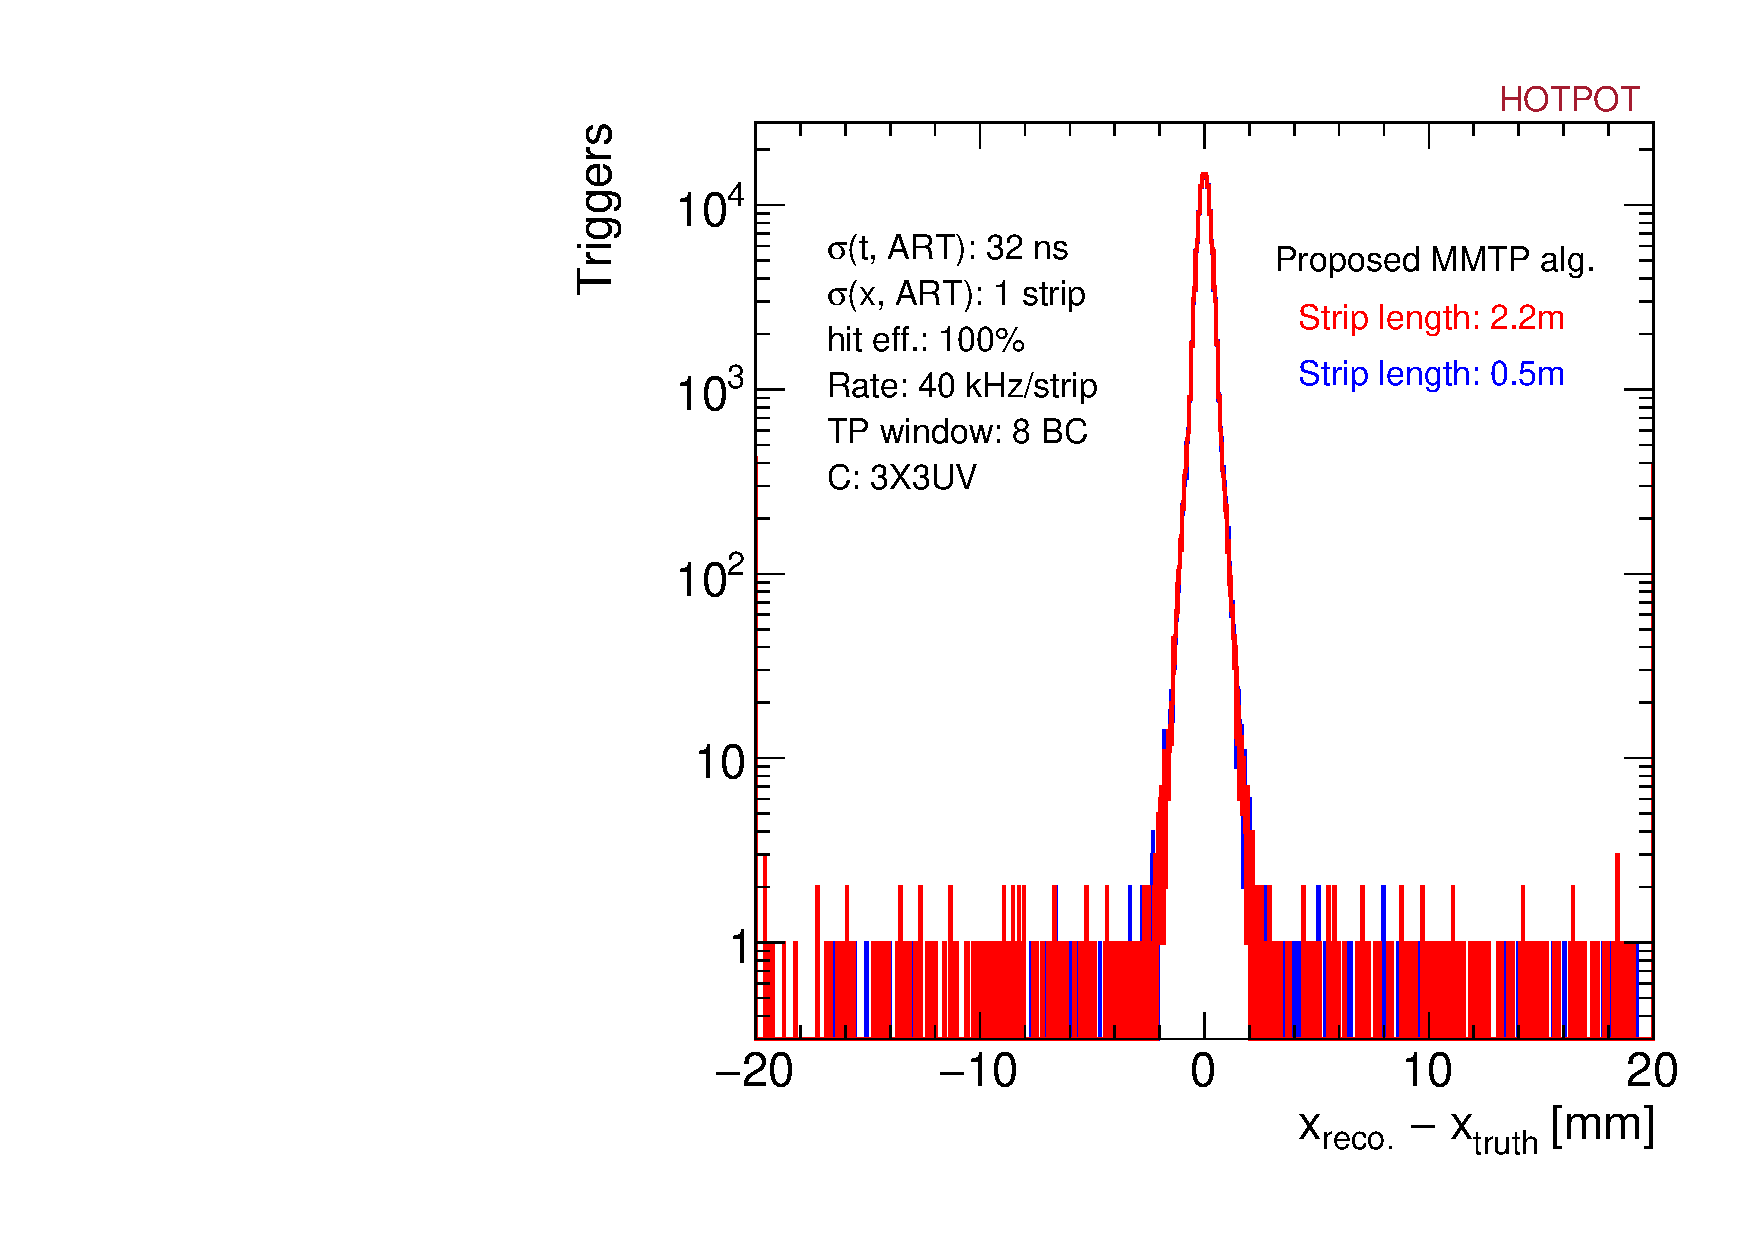
\includegraphics[width=0.48\textwidth]{figures/xres_new.pdf}
    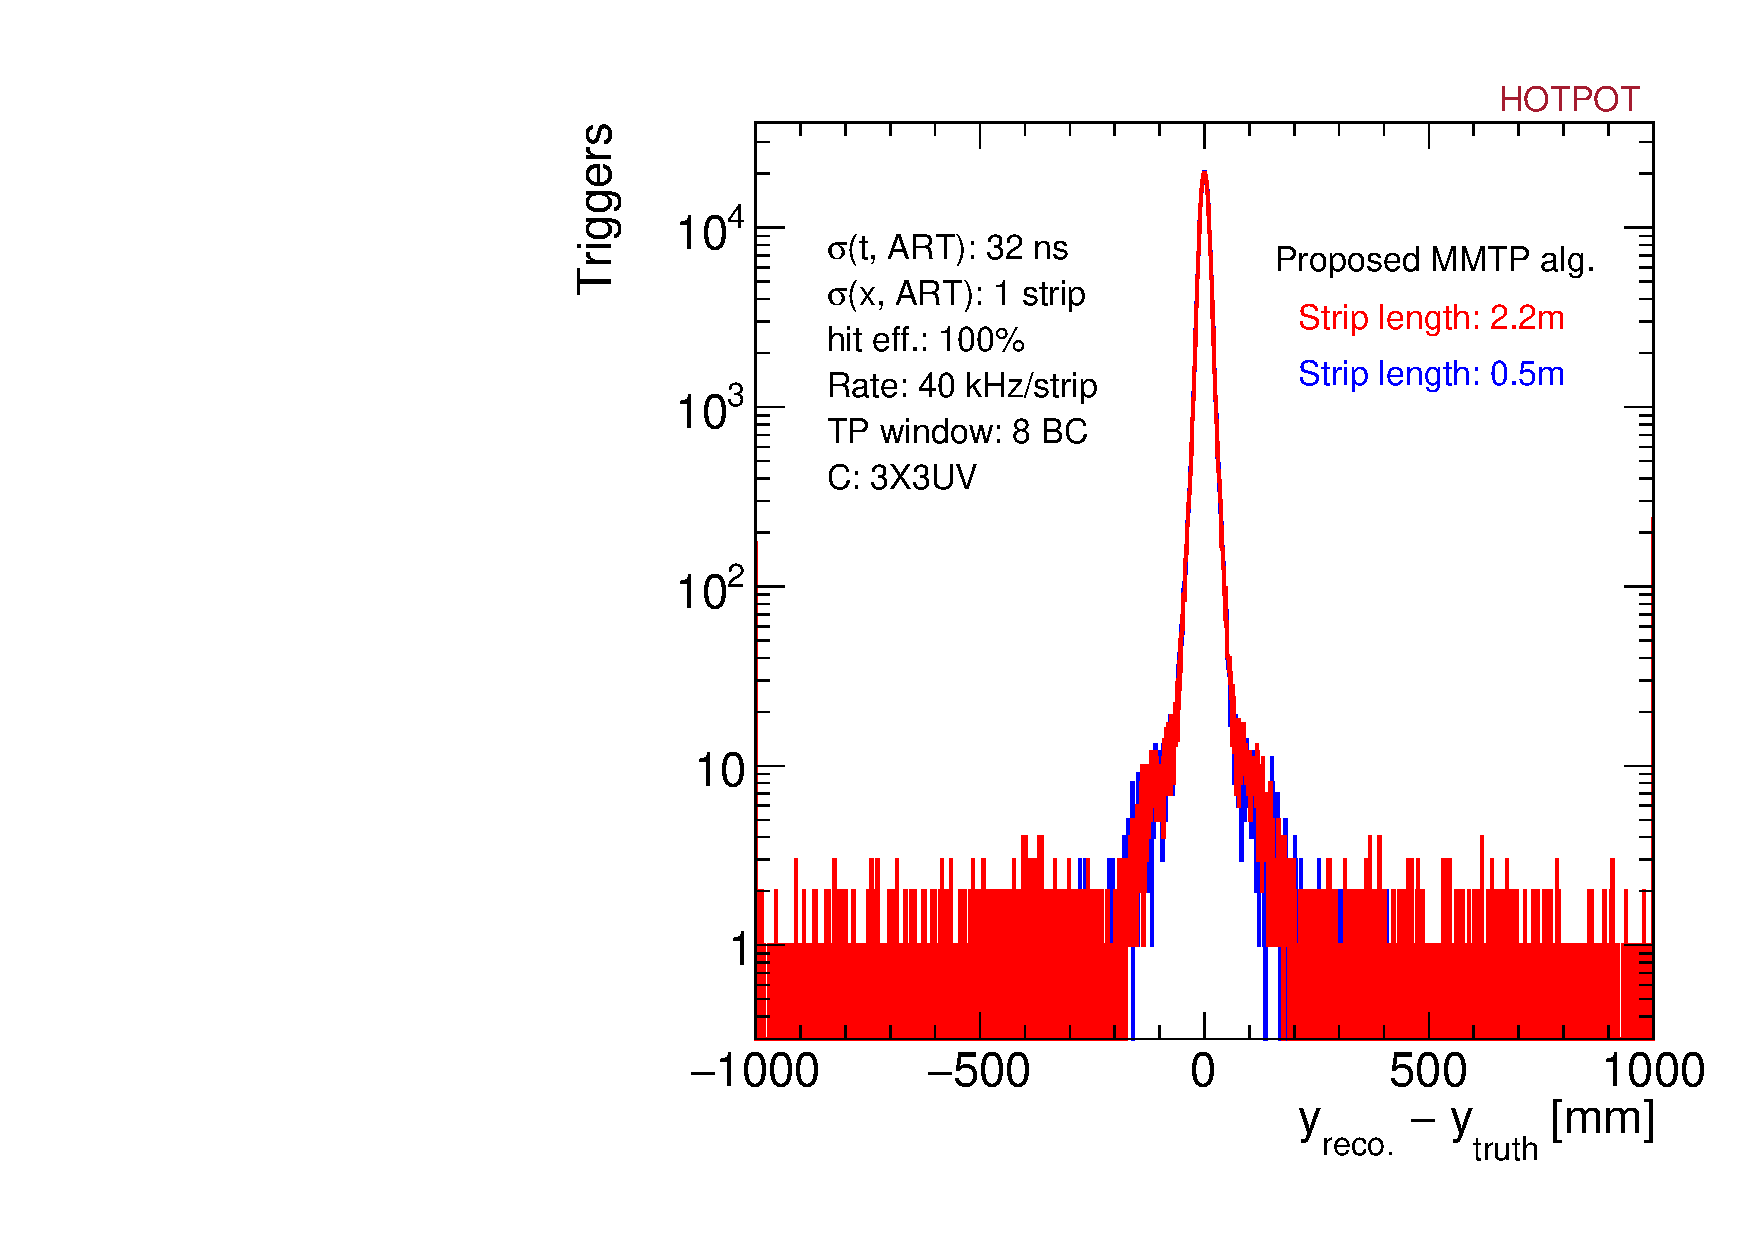
\includegraphics[width=0.48\textwidth]{figures/yres_new.pdf}
    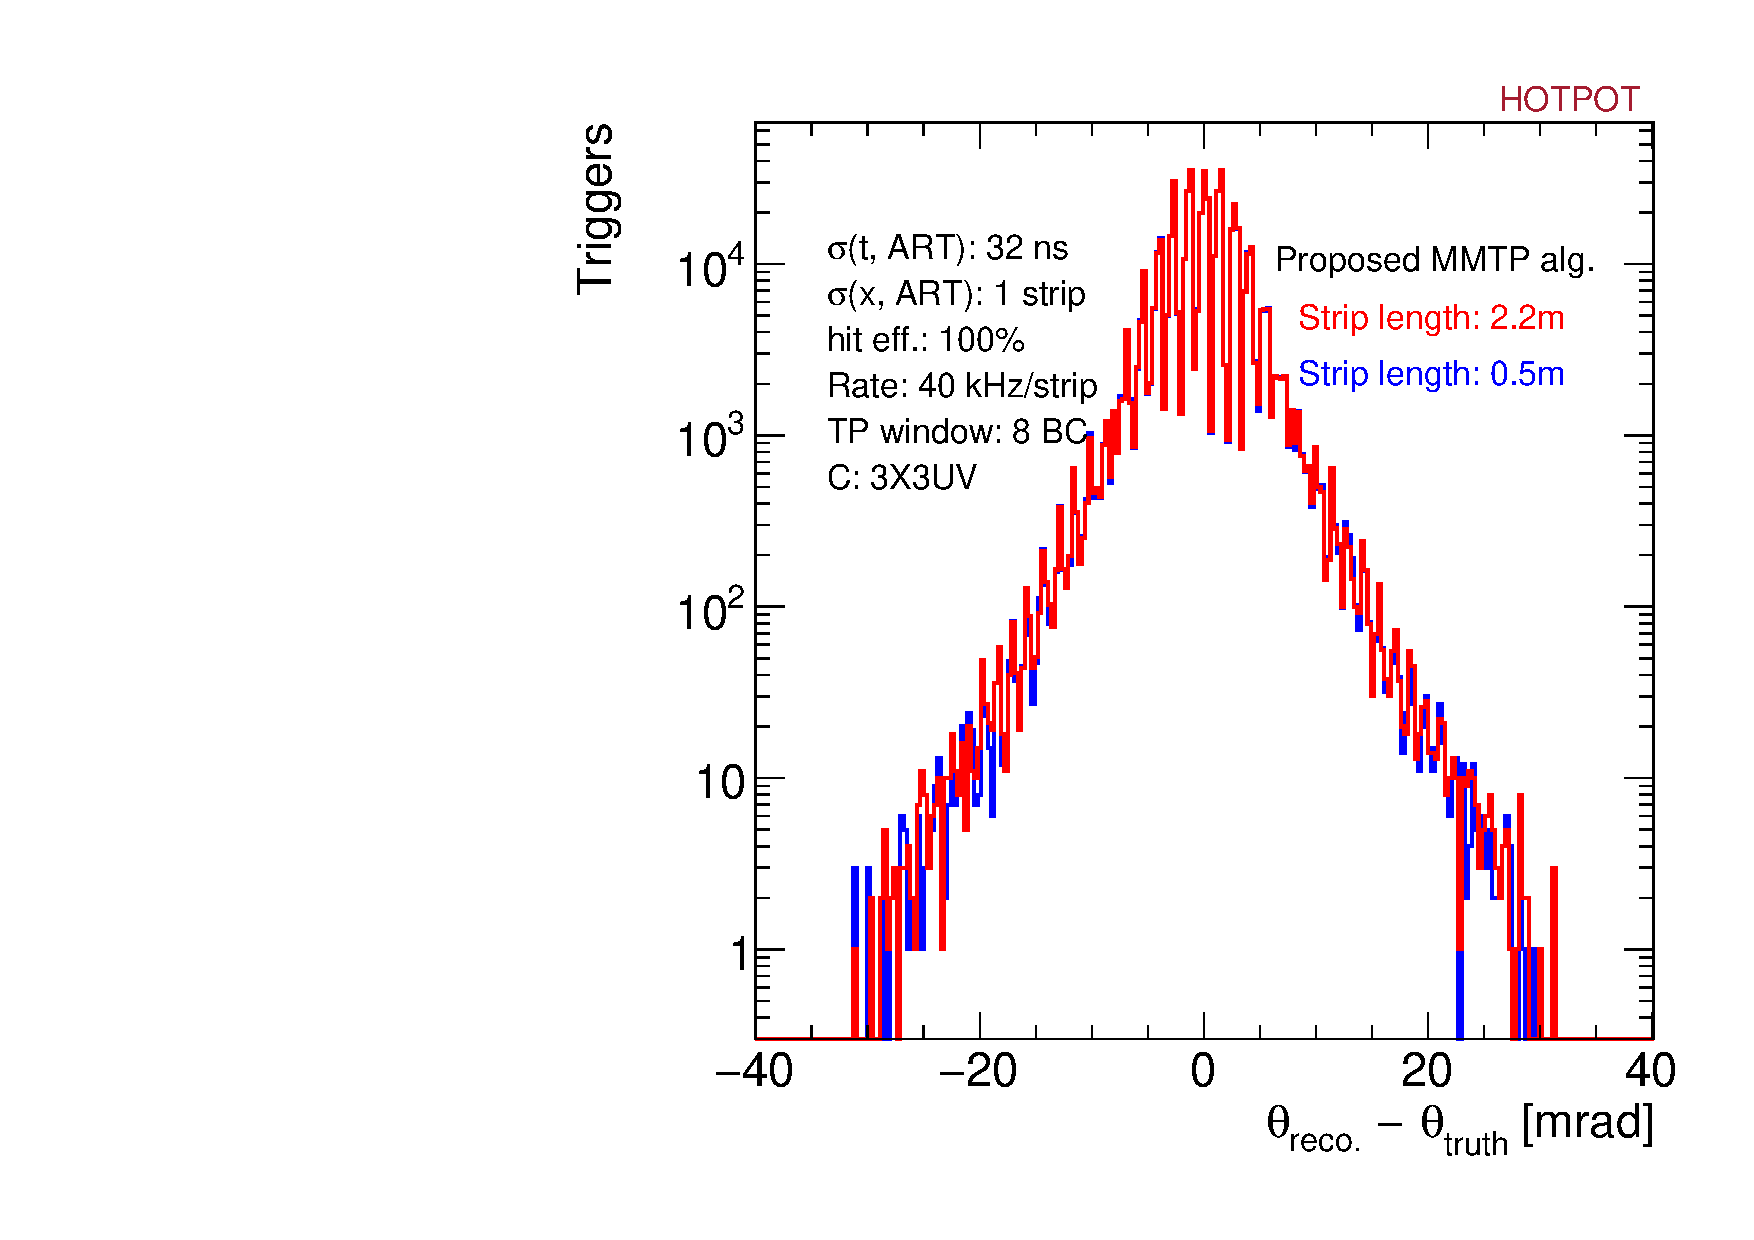
\includegraphics[width=0.48\textwidth]{figures/mres_new.pdf}
  \end{center}
  \vspace{-10pt}
  \caption{Distribution of $x_\text{reco.} - x_\text{truth}$ (top, left), $y_\text{reco.} - y_\text{truth}$ (top, right) and $\theta_\text{reco.} - \theta_\text{truth}$ (bottom) for the proposed MMTP algorithm with uncorrelated background at a rate of 40 kHz per strip.}
  \label{fig:resolutions_new}
\end{figure}

\begin{figure}[!htpb]
  \begin{center}
    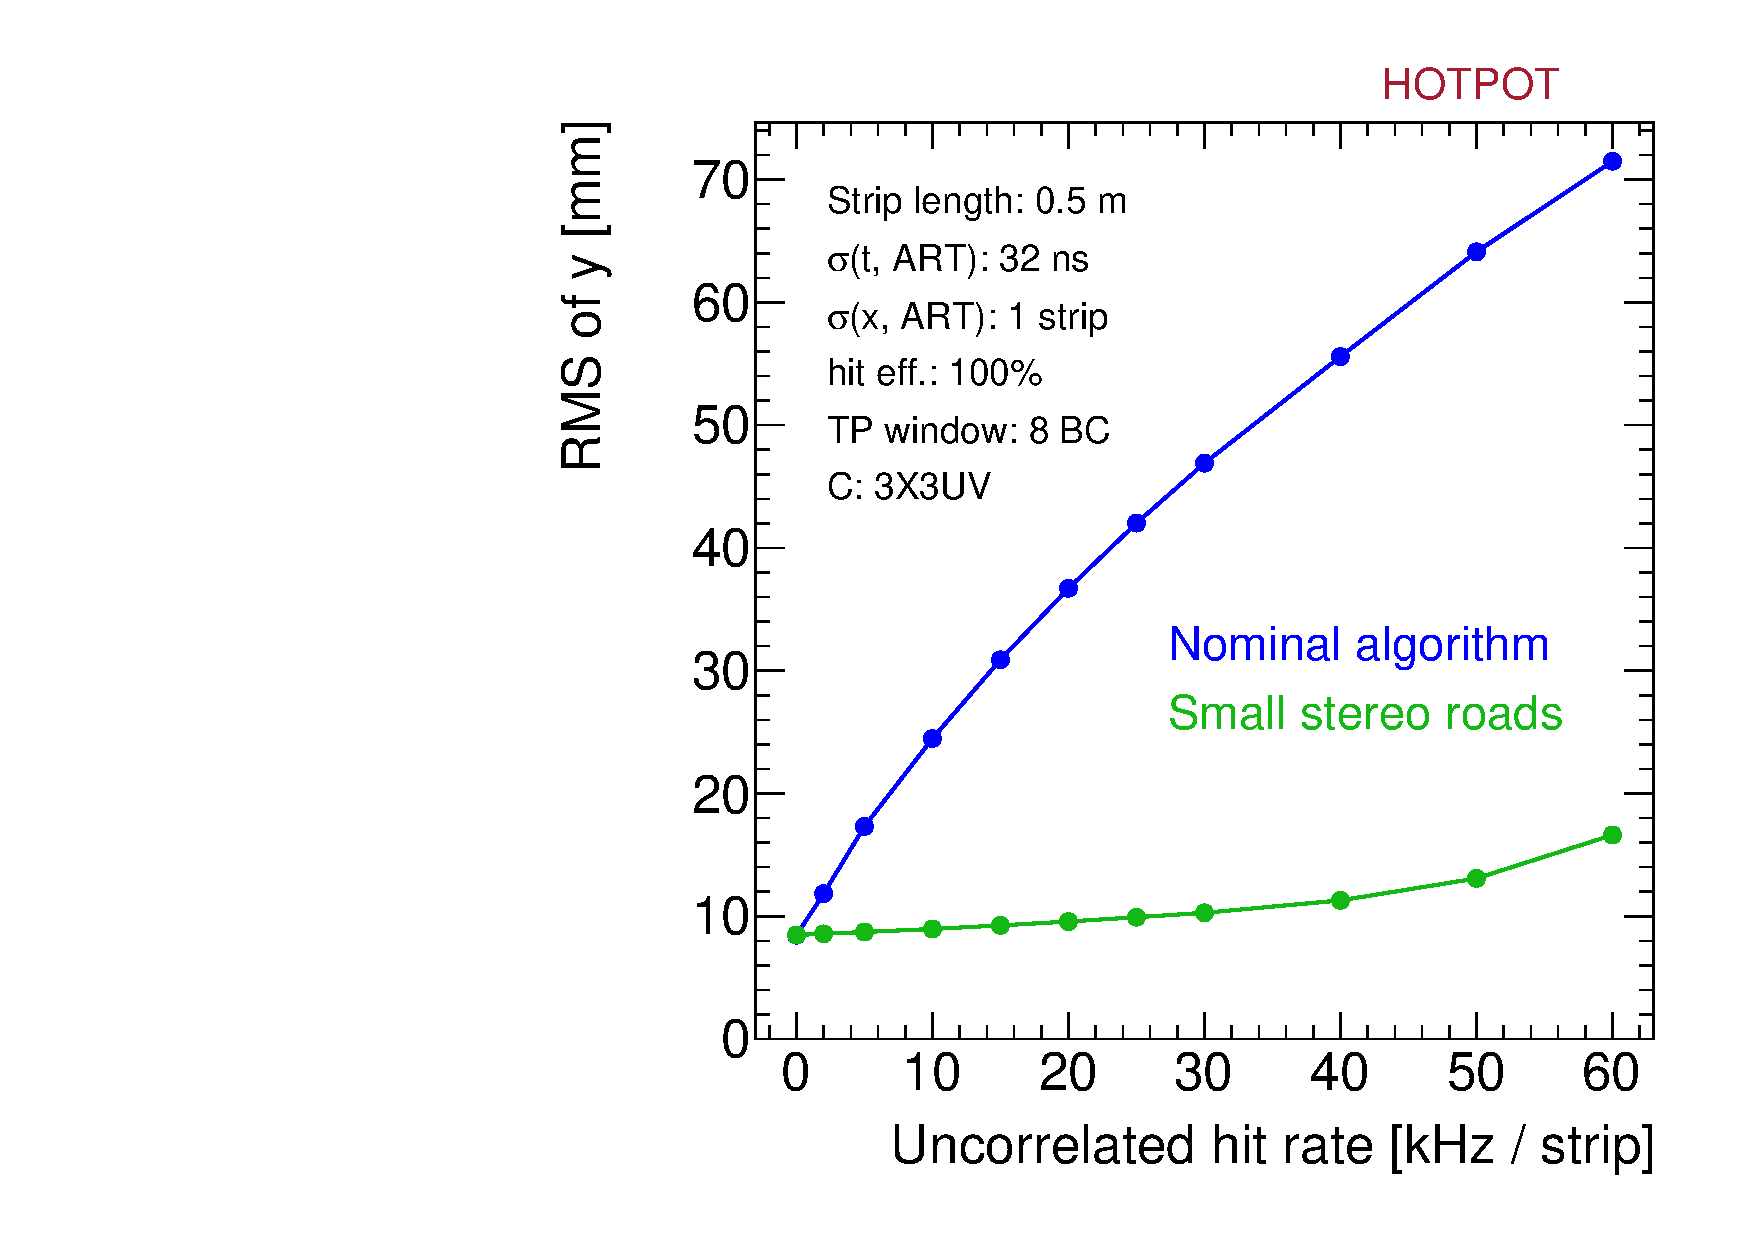
\includegraphics[width=0.48\textwidth]{figures/rms_y_small_vs_rate.pdf}
    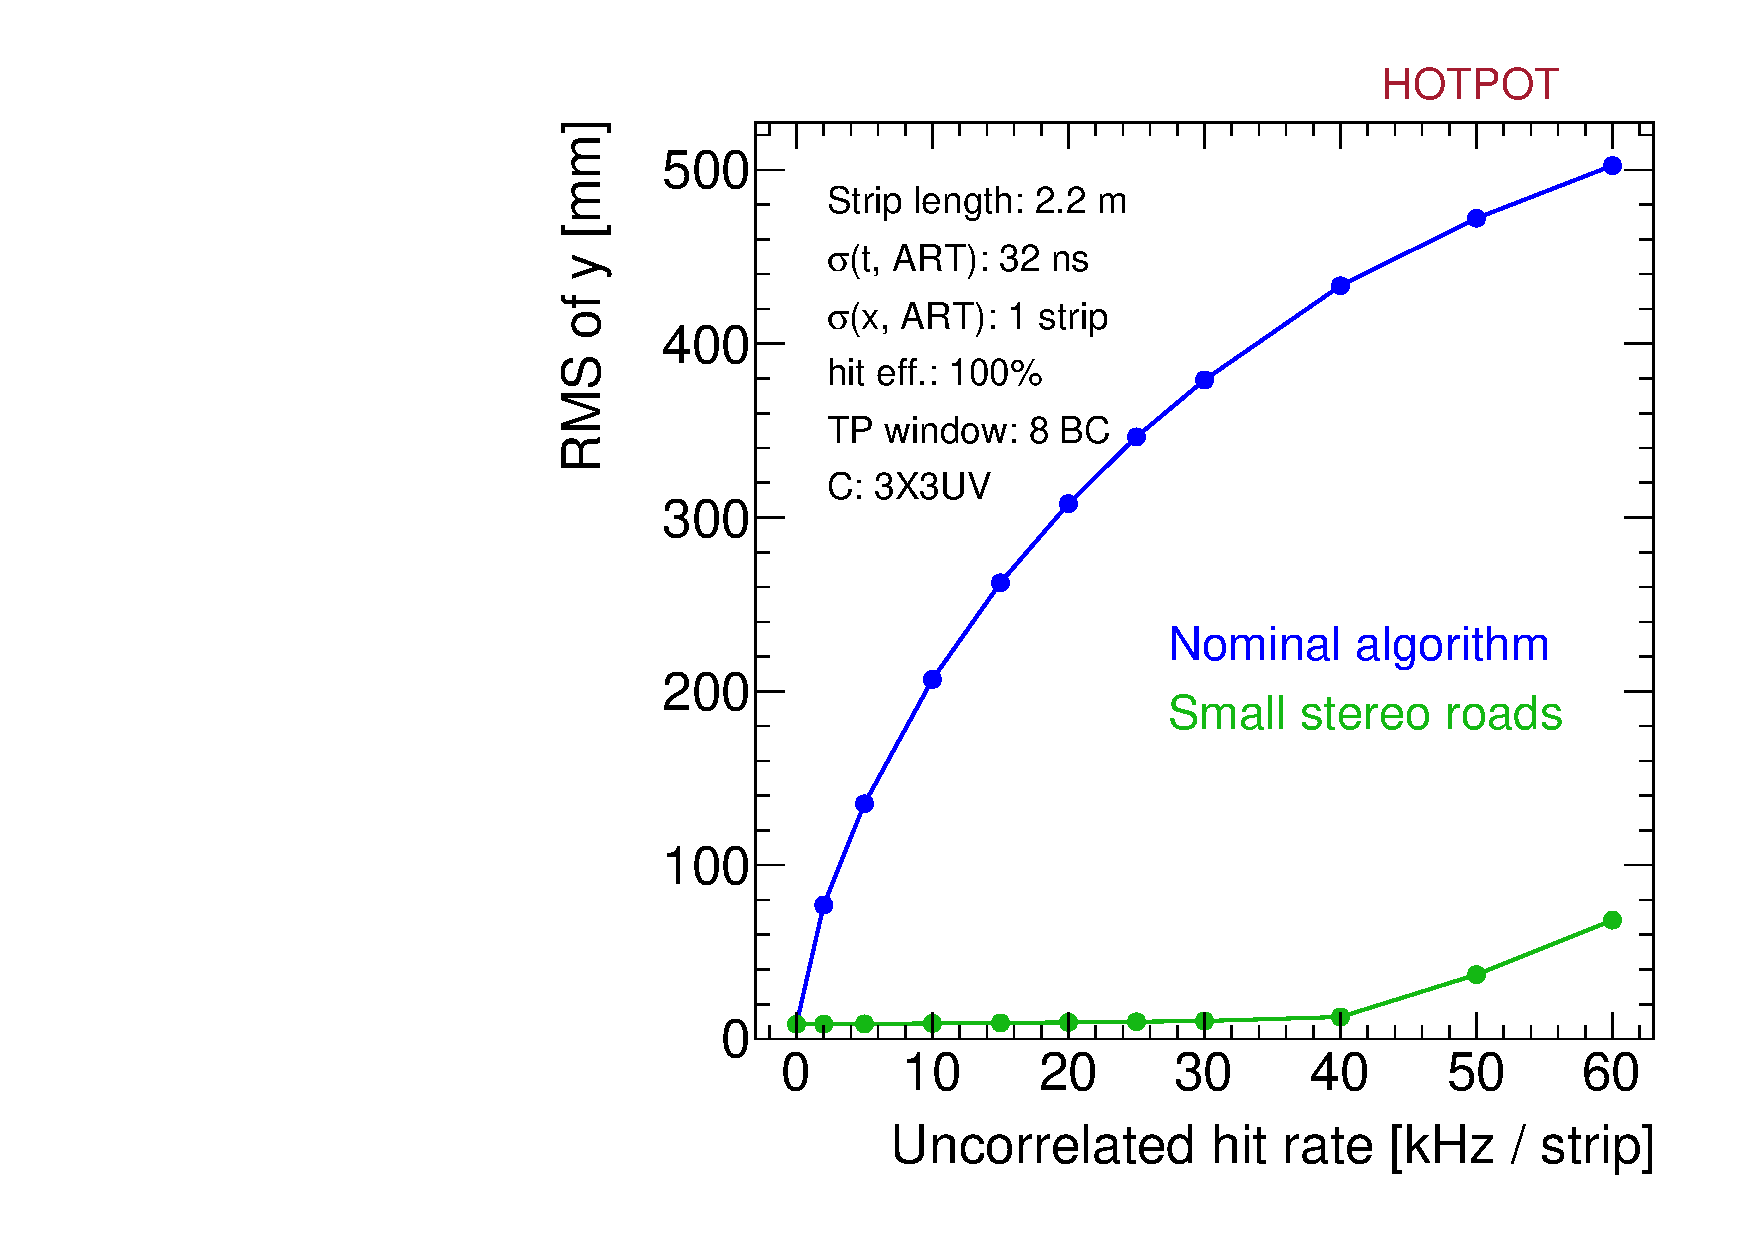
\includegraphics[width=0.48\textwidth]{figures/rms_y_large_vs_rate.pdf}
  \end{center}
  \vspace{-10pt}
  \caption{RMS of $y_\text{reco.} - y_\text{truth}$ for a strip size of 0.5m (left) and 2.2m (right) as a function of uncorrelated background rate. The RMS is calculated in the $3\sigma$ (99.7\%) range of the distribution.}
  \label{fig:rms_vs_rate}
\end{figure}

\begin{figure}[!htpb]
  \begin{center}
    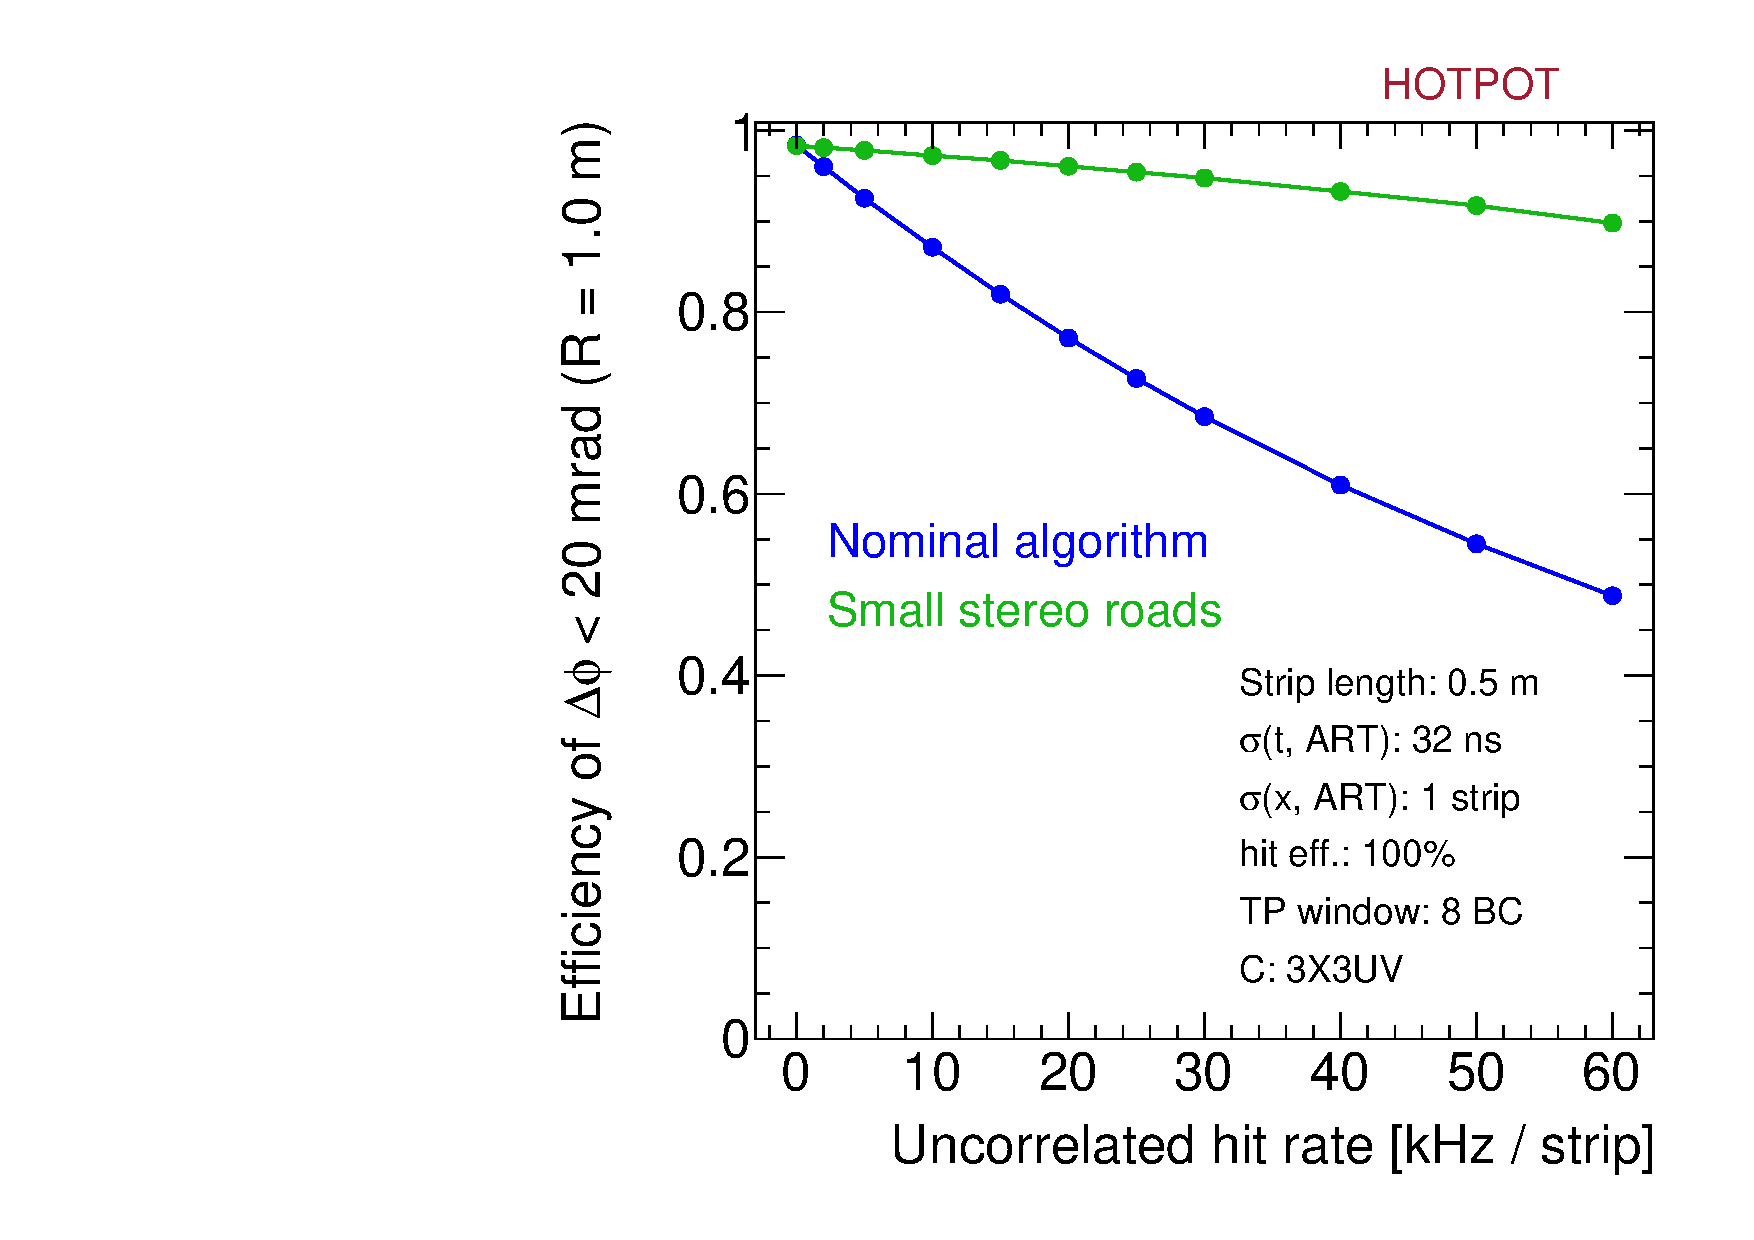
\includegraphics[width=0.48\textwidth]{figures/eff_phi_small_vs_rate.pdf}
    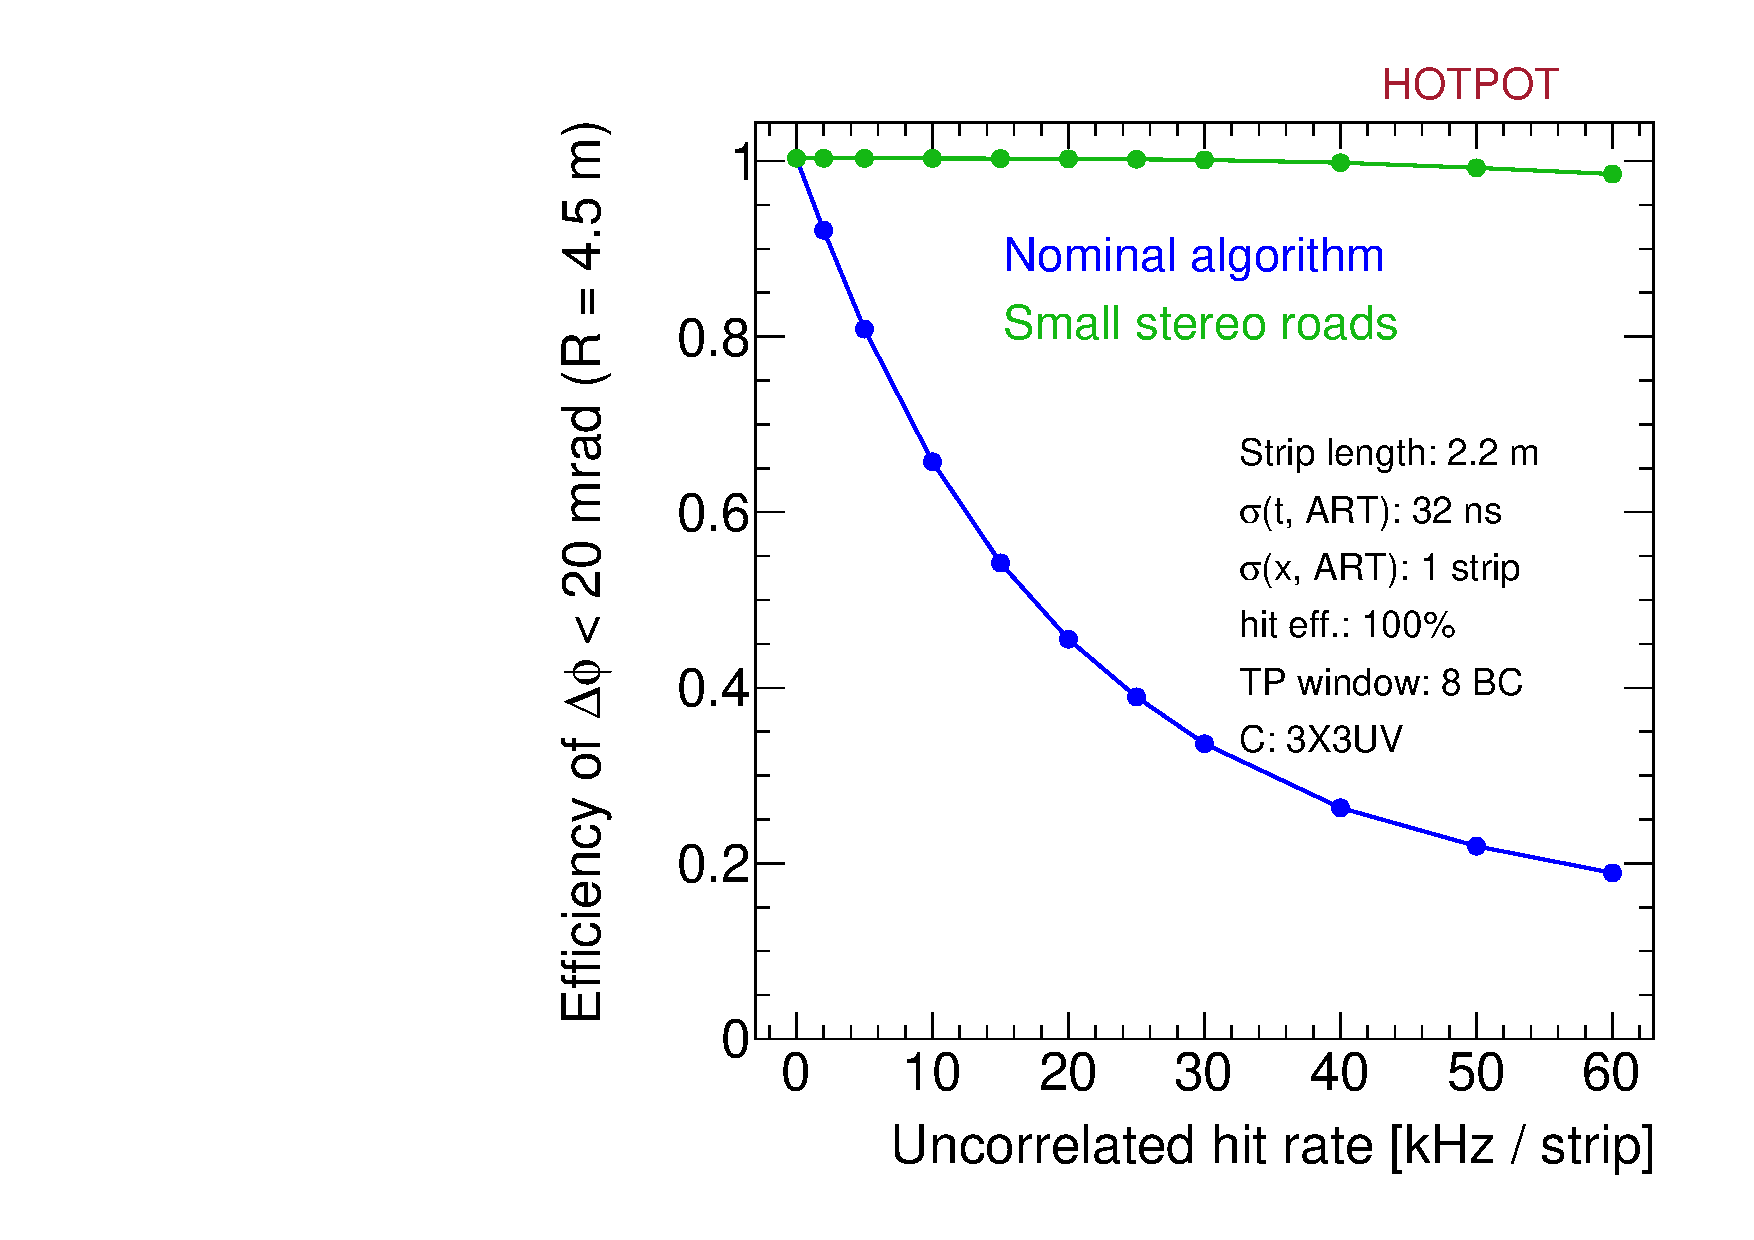
\includegraphics[width=0.48\textwidth]{figures/eff_phi_large_vs_rate.pdf}
  \end{center}
  \vspace{-10pt}
  \caption{Efficiency of $\phi_\text{reco.} - \phi_\text{truth} < 20$ mrad for a strip size of 0.5m (left) and 2.2m (right). $\phi_\text{reco.}-\phi_\text{truth}$ is calculated as $\frac{y_\text{reco.} - y_\text{truth}}{R}$, where $R$ is the distance from the beamline. $R$ is taken to be 1m for the small chamber and 4.5m for the large chamber.}
  \label{fig:eff_vs_rate}
\end{figure}


\section{Absolute road coordinates}
\label{sec:roadcoord}

Because of limitations in hardware FPGA resources, calculating an (x,y) position with the ART hits in a road may be costly. To save resources, if we have small roads, i.e. 8-strip $X$,$U$,$V$ roads, we can assign an absolute (x,y) position to each unique set of $X$,$U$,$V$ roads. This is the position of the center of the diamond shown in Figure \ref{fig:cartoon_smallroads_1}. In the FPGA implementation, this would be reduced to a set of lookup tables. The performance of this is given in Figure \ref{fig:resolutions_cen}. This performs noticeably worse than using the ART strips in a road to calculate a position. The 3$\sigma$ y-residual RMS is 32.38 (33.45) $\pm$ 0.03 (0.03) mm for 0.5m (2.2m) long strips, which is about a factor of 3 worse than the calculation with strips. The 3$\sigma$ x-residual RMS is 0.07959 (0.7965) $\pm$ 0.0008 (0.0008) mm for 0.5m (2.2m) long strips. Using the strips, the x-residual RMS is 0.2969 (0.3019) $\pm$ 0.0003 (0.0003) mm for 0.5m (2.2m) long strips. However, with the added effect of $\delta$-rays, which we cannot simulate here, these two methods may be comparable.  

\begin{figure}[!htpb]
  \begin{center}
    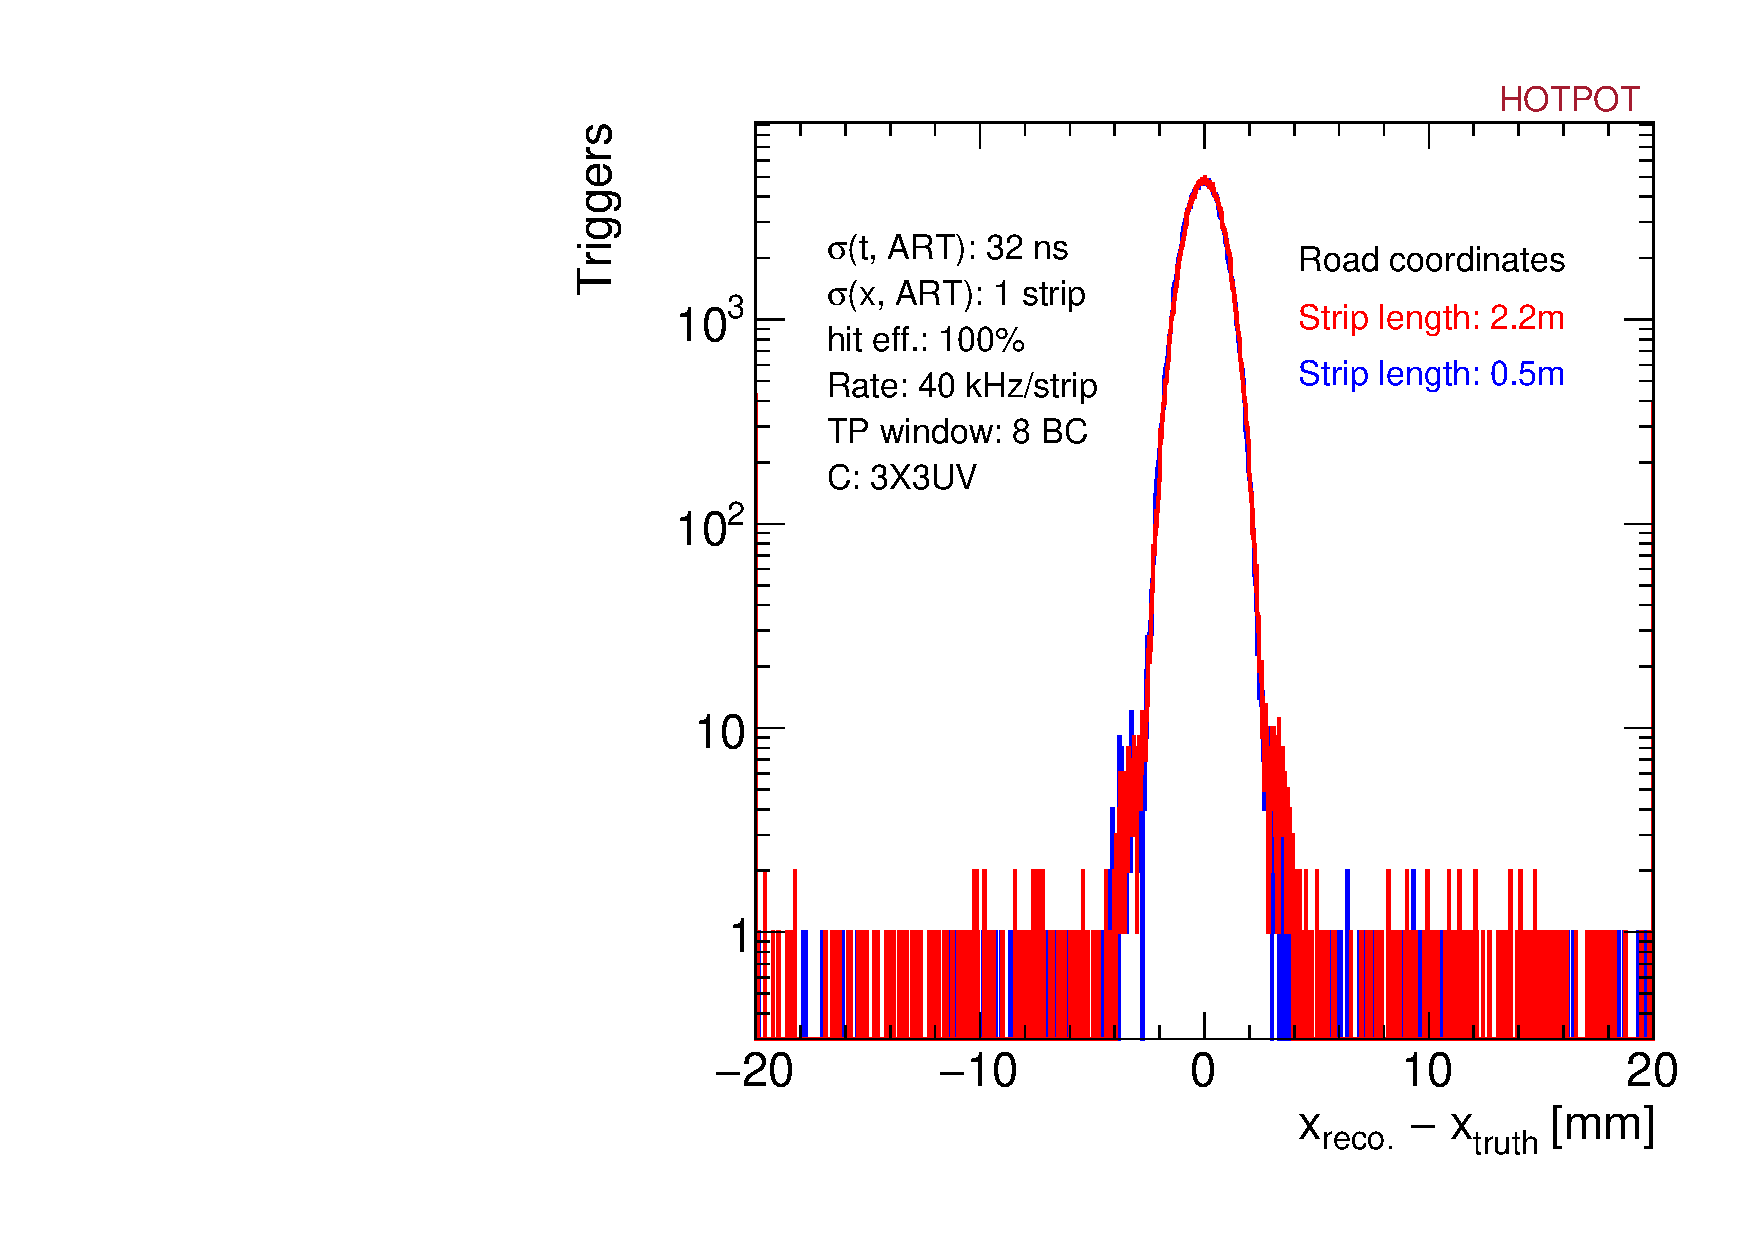
\includegraphics[width=0.48\textwidth]{figures/xres_cen.pdf}
    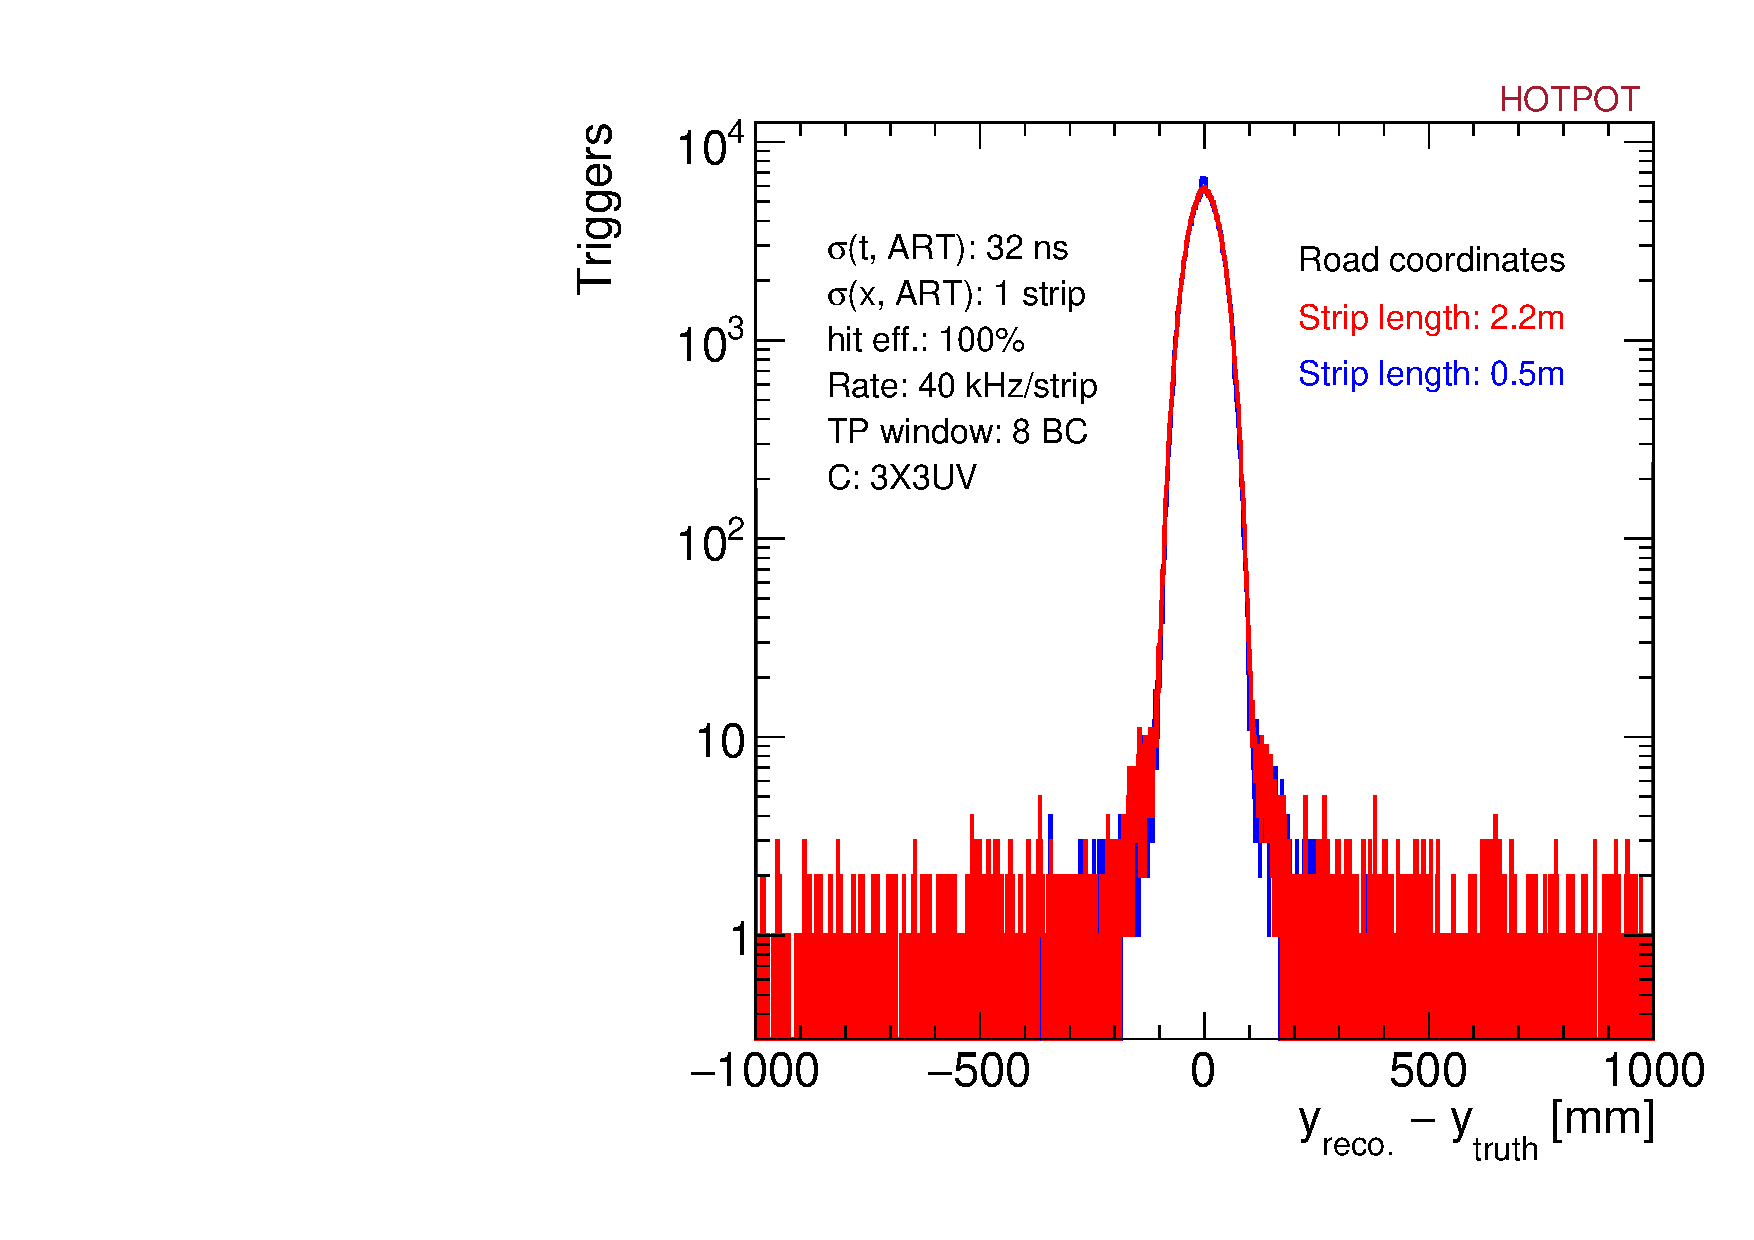
\includegraphics[width=0.48\textwidth]{figures/yres_cen.pdf}
  \end{center}
  \vspace{-10pt}
  \caption{Distribution of $x_\text{reco.} - x_\text{truth}$ (left) and $y_\text{reco.} - y_\text{truth}$ (right) for the proposed MMTP algorithm, where each unique set of $X$,$U$,$V$ roads is assigned a (x,y) position, with uncorrelated background at a rate of 40 kHz per strip.}
  \label{fig:resolutions_cen}
\end{figure}

\section{Trigger rate}
\label{sec:trigrate}

Although the proposed algorithm rescues the y-resolution, the presence of the extra roads in the $U$,$V$ planes greatly increases the number of triggers found per BC. Under high background conditions, the MMTP cannot be a standalone trigger. With 2.2m (0.5m) long strips and an implementation region of 136 (96) roads, we have an average of 0.02 (0.004) triggers per BC with 40 kHz/strip of background. This averages to be about 0.3 triggers per BC in the entire NSW. 
\par To meet latency and resource requirements, the number of triggers that need to be processed must be as small as possible. Processing 1-2 triggers per BC is easily managed by the MMTP. However, the number of triggers per BC spikes when a muon passes through. Without any background hits, each hit can satisfy up one or two $X$, $U$, or $V$ roads with the neighboring-road effect, and therefore we can can make up to 6 triggers per BC. When the background hits are added, this number can go up to 15 triggers per BC, as shown in Fig. \ref{fig:ntrig}. Note that the distribution of the number of triggers in a given BC depends on which BC you are looking at. Fig. \ref{fig:ntrig} shows the distribution of the number of triggers for \textit{one} BC. We look at the BC in which the first real muon hit has been in the MMTP buffer for 8 BCs. This is the BC with the highest average number of triggers.
\par It is unclear how to process all of these triggers in a timely fashion in the FPGA. This is to be determined.
\begin{figure}[!htpb]
  \begin{center}
    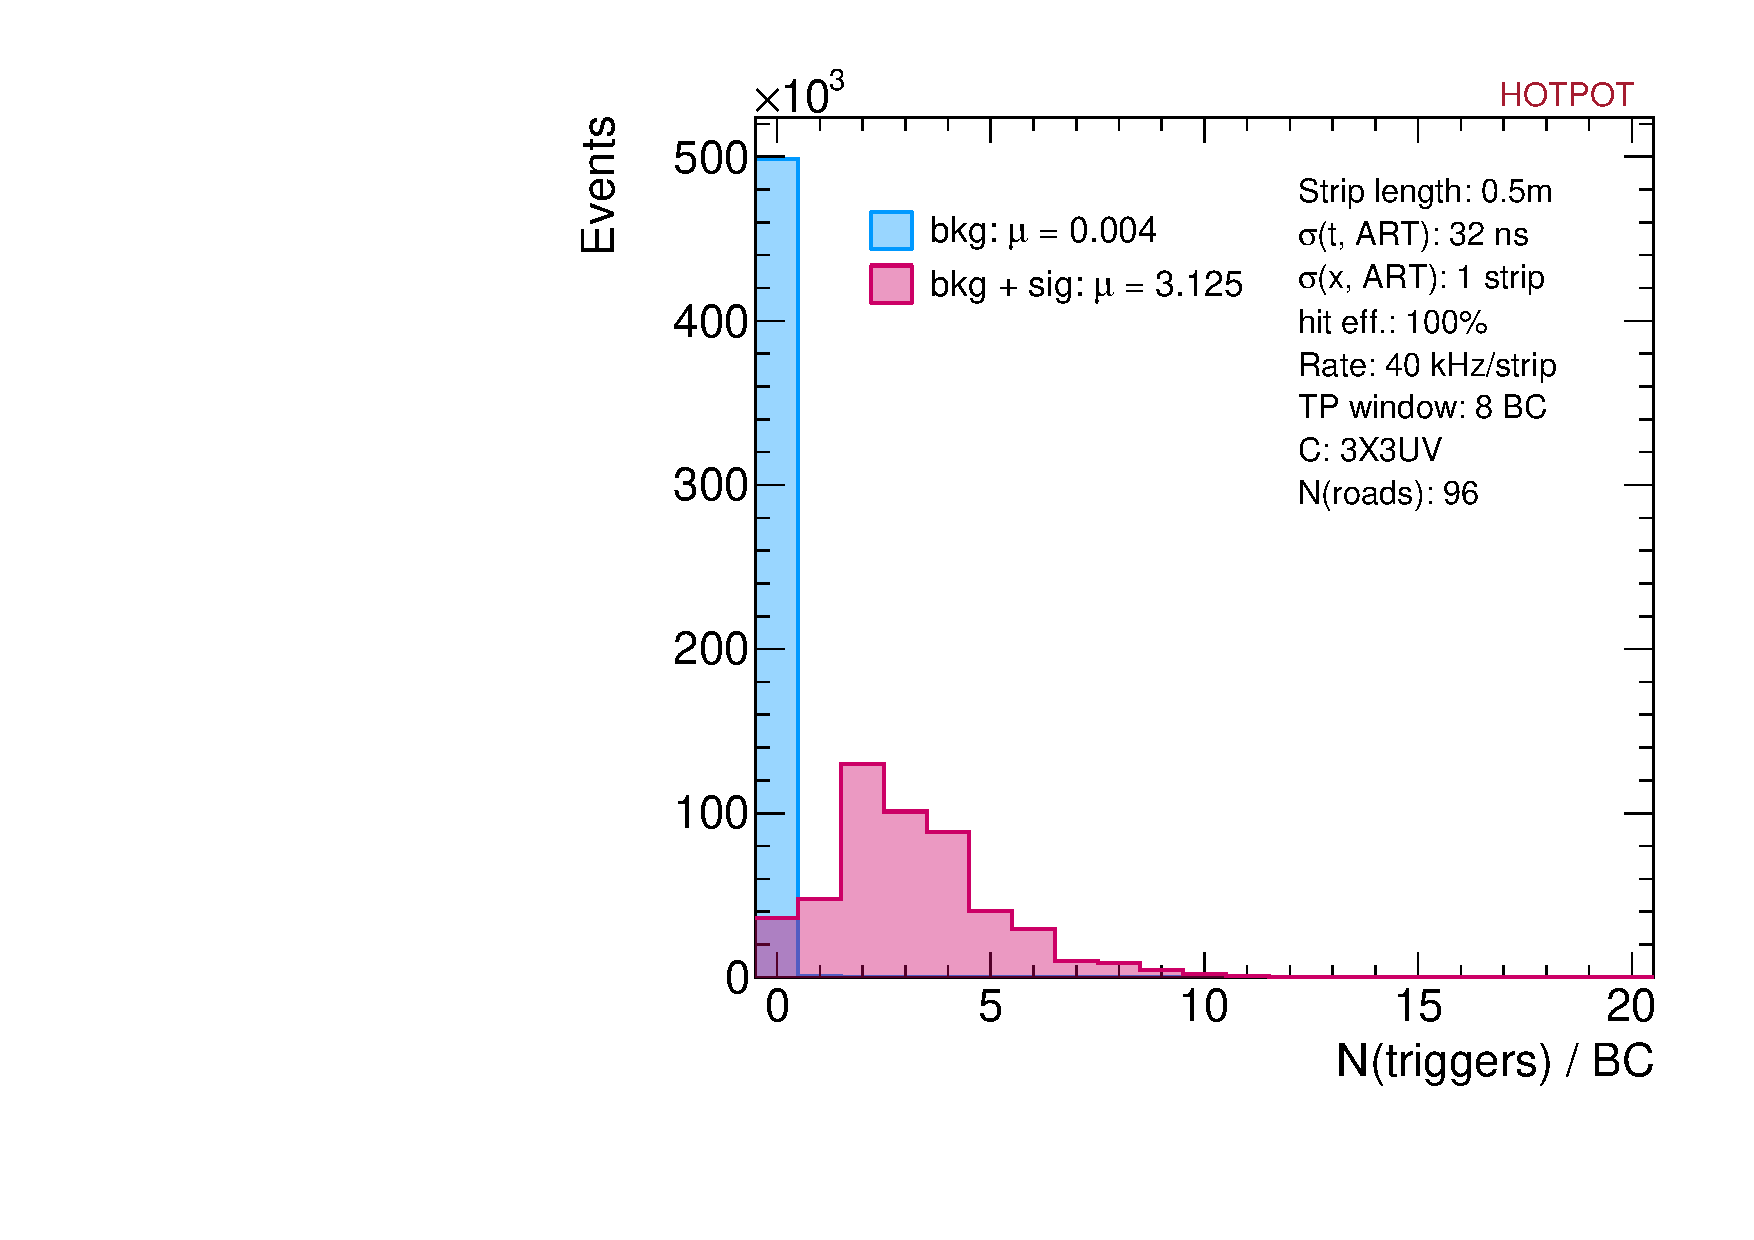
\includegraphics[width=0.48\textwidth]{figures/r96_ntrig_BC7.pdf}
    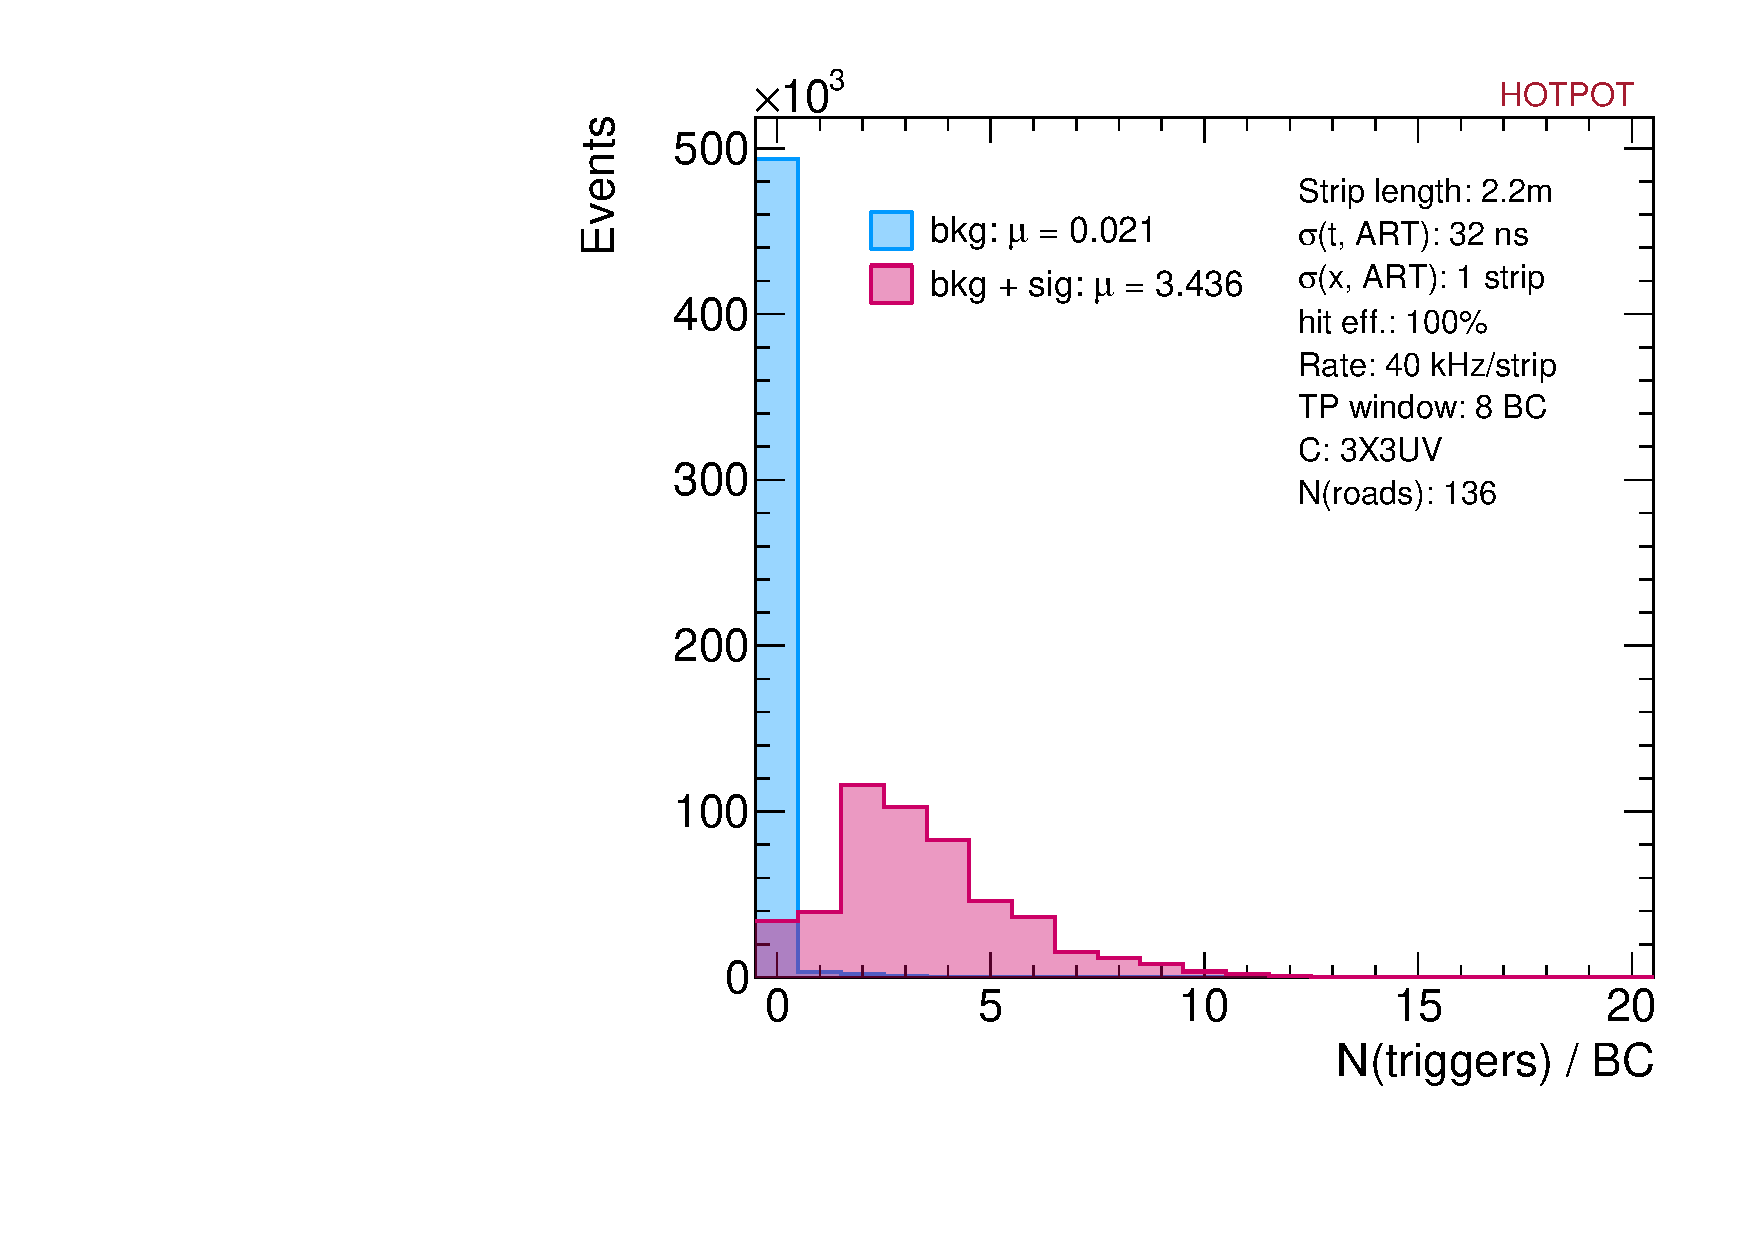
\includegraphics[width=0.48\textwidth]{figures/r136_ntrig_BC7.pdf}
  \end{center}
  \vspace{-10pt}
  \caption{Number of triggers found per BC for 0.5m long strips (left) and 2.2m long strips (right). The blue histogram represents the distribution if we only have uncorrelated background hits, and the pink histogram represents the distribution if we also add a muon track. For the pink histogram, since number of triggers in a given BC is dependent on the BC, we pick the BC when the first real muon ART hit is 8 BCs old.}
  \label{fig:ntrig}
\end{figure}

\section{Multistage architecture}
\label{sec:multistage}

\begin{figure}[!htpb]
  \begin{center}
    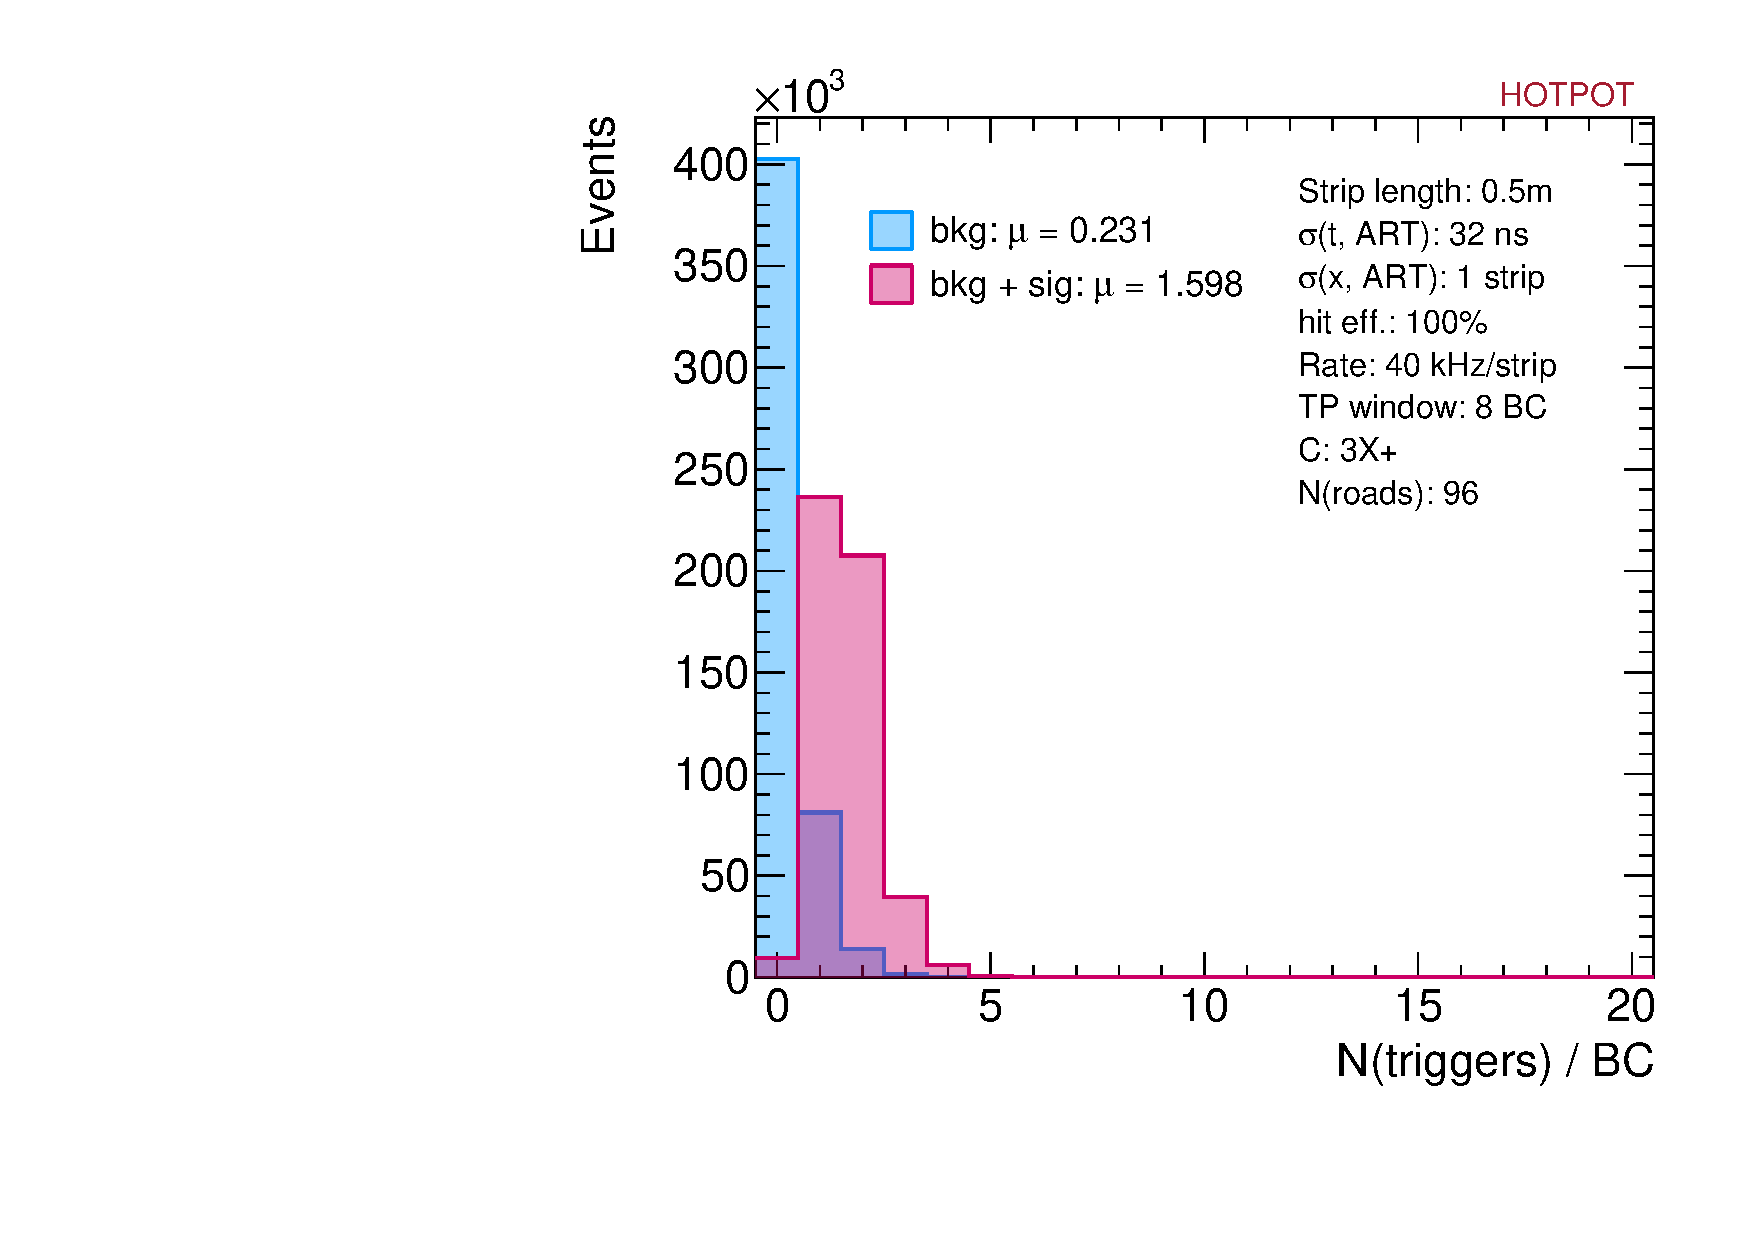
\includegraphics[width=0.48\textwidth]{figures/small_3x0uv_ntrig_BC7.pdf}
    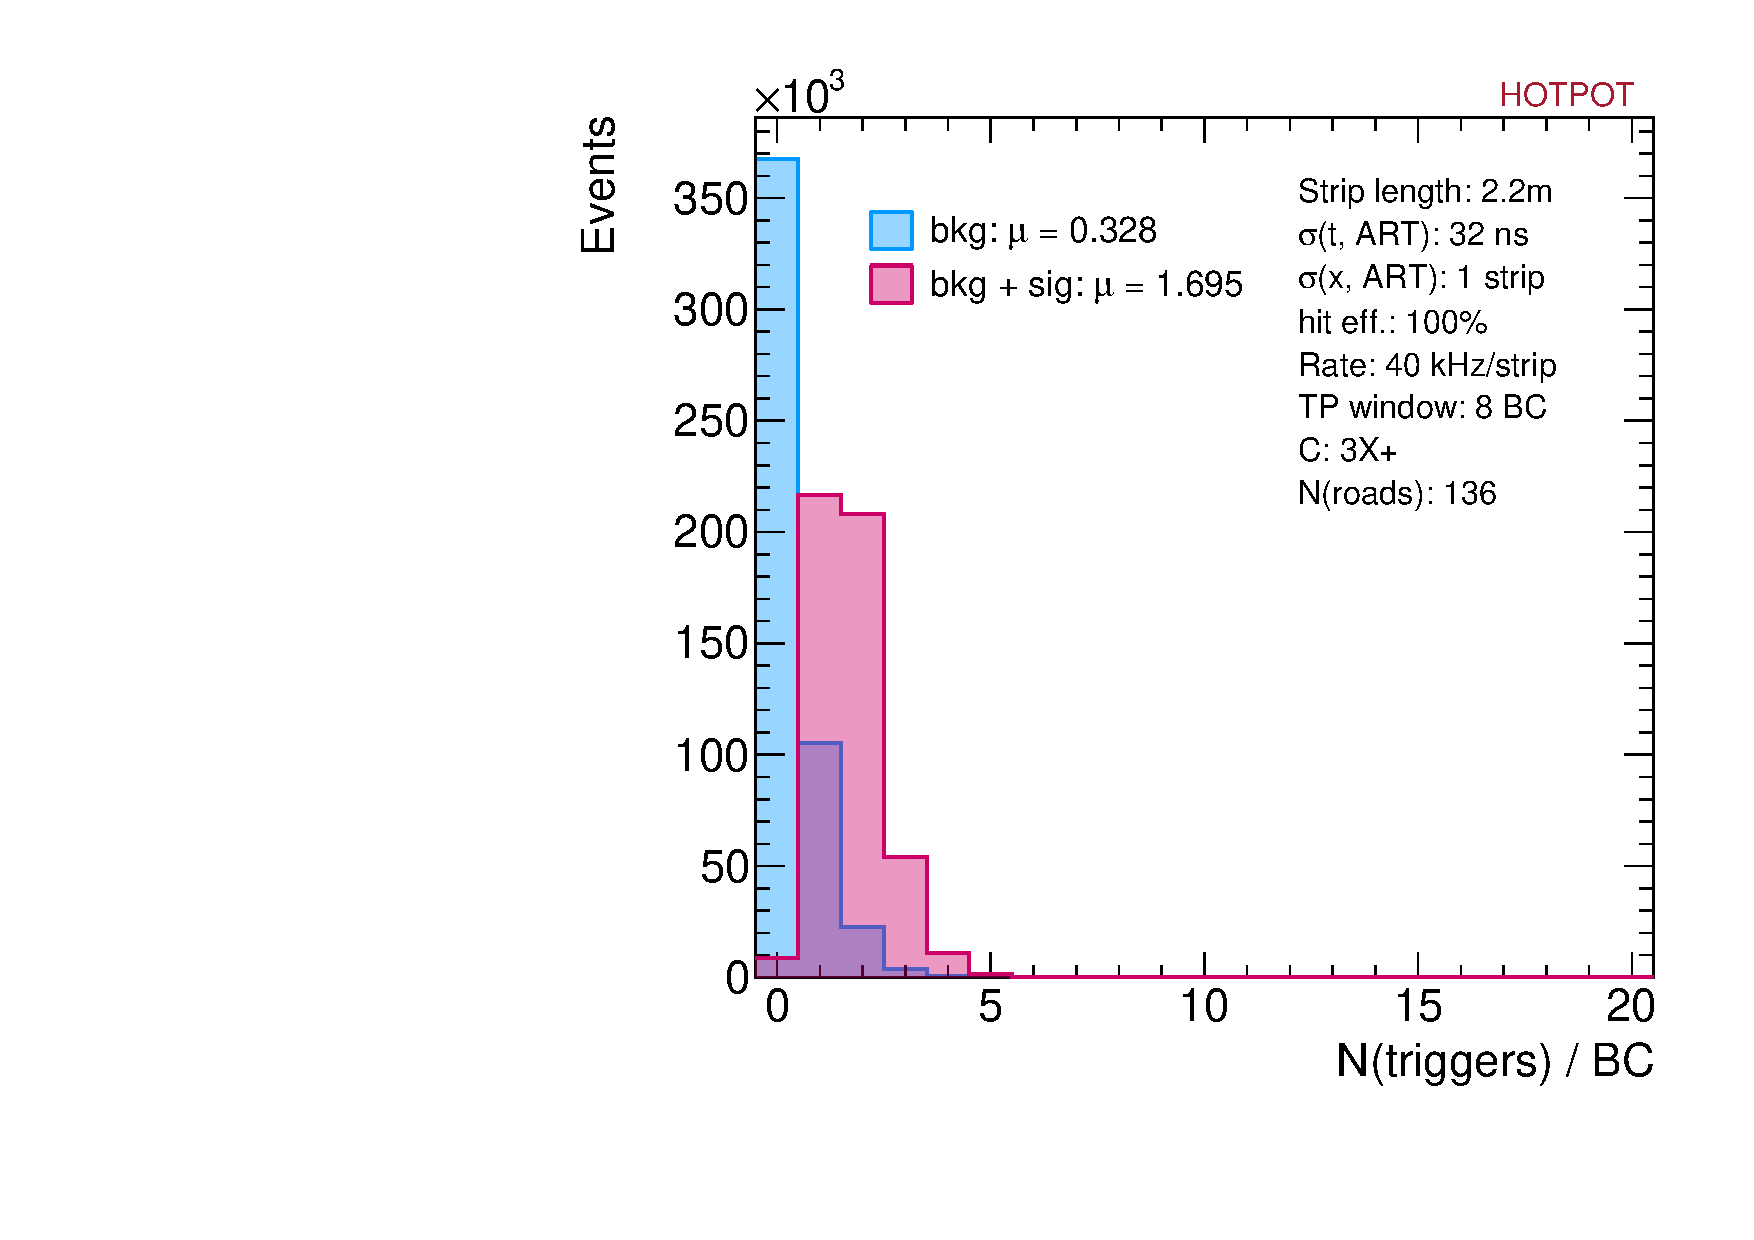
\includegraphics[width=0.48\textwidth]{figures/large_3x0uv_ntrig_BC7.pdf}
  \end{center}
  \vspace{-10pt}
  \caption{Number of triggers found per BC for 0.5m long strips (left) and 2.2m long strips (right) with a 3X requirement. The blue histogram represents the distribution if we only have uncorrelated background hits, and the pink histogram represents the distribution if we also add a muon track. For the pink histogram, since number of triggers in a given BC is dependent on the BC, we pick the BC when the first real muon ART hit is 8 BCs old.}
  \label{fig:3x_trig}
\end{figure}

With the proposed algorithm modifications using small stereo roads, a multistage trigger finder is currently implemented to reduce redundant processing. In order to avoid the scaling of having many unique pairs of $U$, $V$ roads per X road, a stage I filter for triggers is applied. In this stage, we look for 3X coincidences with no requirement on the ages of the ART hits. This narrows the set of X roads. Then, in stage II, we look for 3X3UV+ coincidences in $U$, $V$ roads associated to the pre-filtered set of X roads. We also require that one of the ART hits is ``mature", or 8 BCs old in the buffer which collects ART hits. The caveat of this multistage filtering setup is that the number of $X$ roads in the pre-filtered set must be limited to a set number, \textit{n}. A similar limit, \textit{m}, also applies to the number of 3X3UV coincidences that can be processed per corresponding X road. $n \times m$ must be fewer than 8, a number which is determined by the mother clock in the MMTP implementation. Figure \ref{fig:mstage} illustrates this scheme.

\begin{figure}[!htpb]
  \begin{center}
    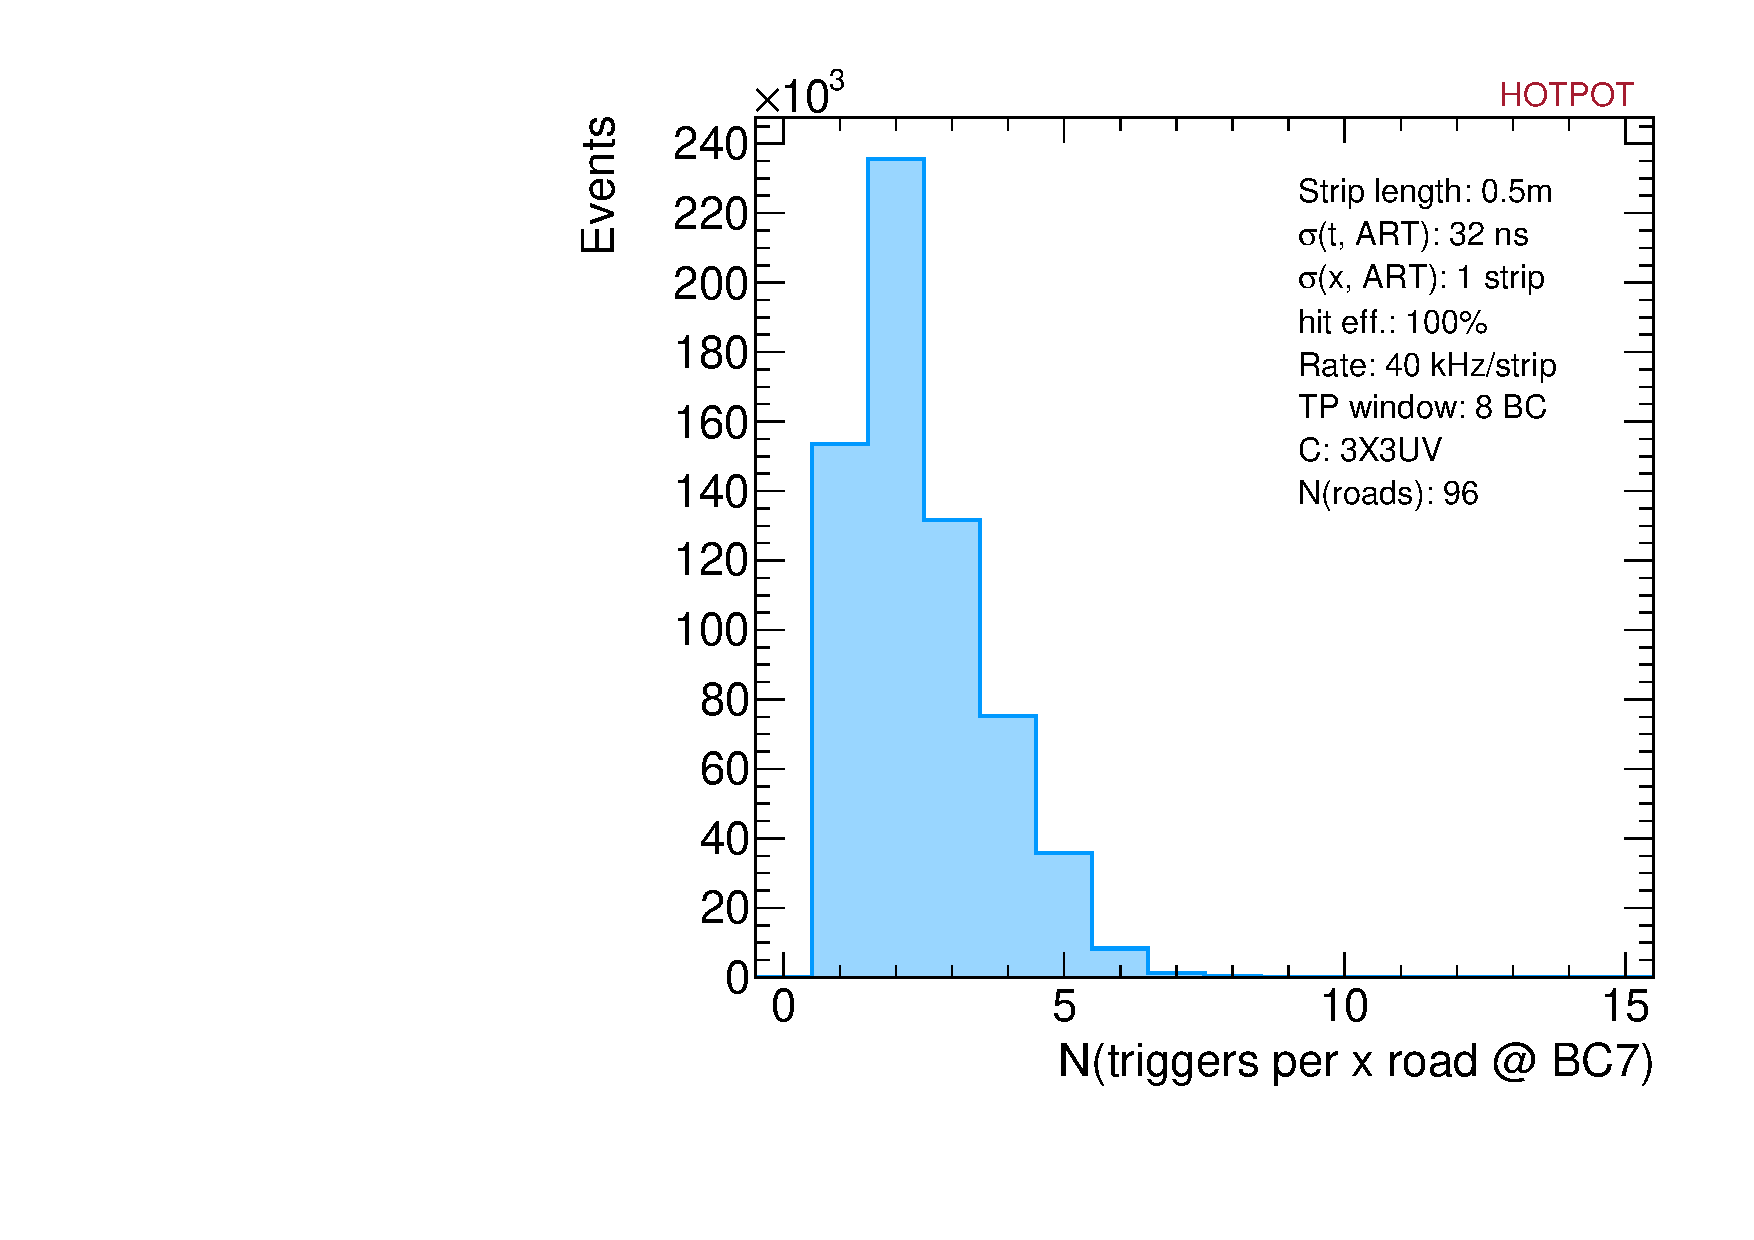
\includegraphics[width=0.48\textwidth]{figures/small_trigs_per_x.pdf}
    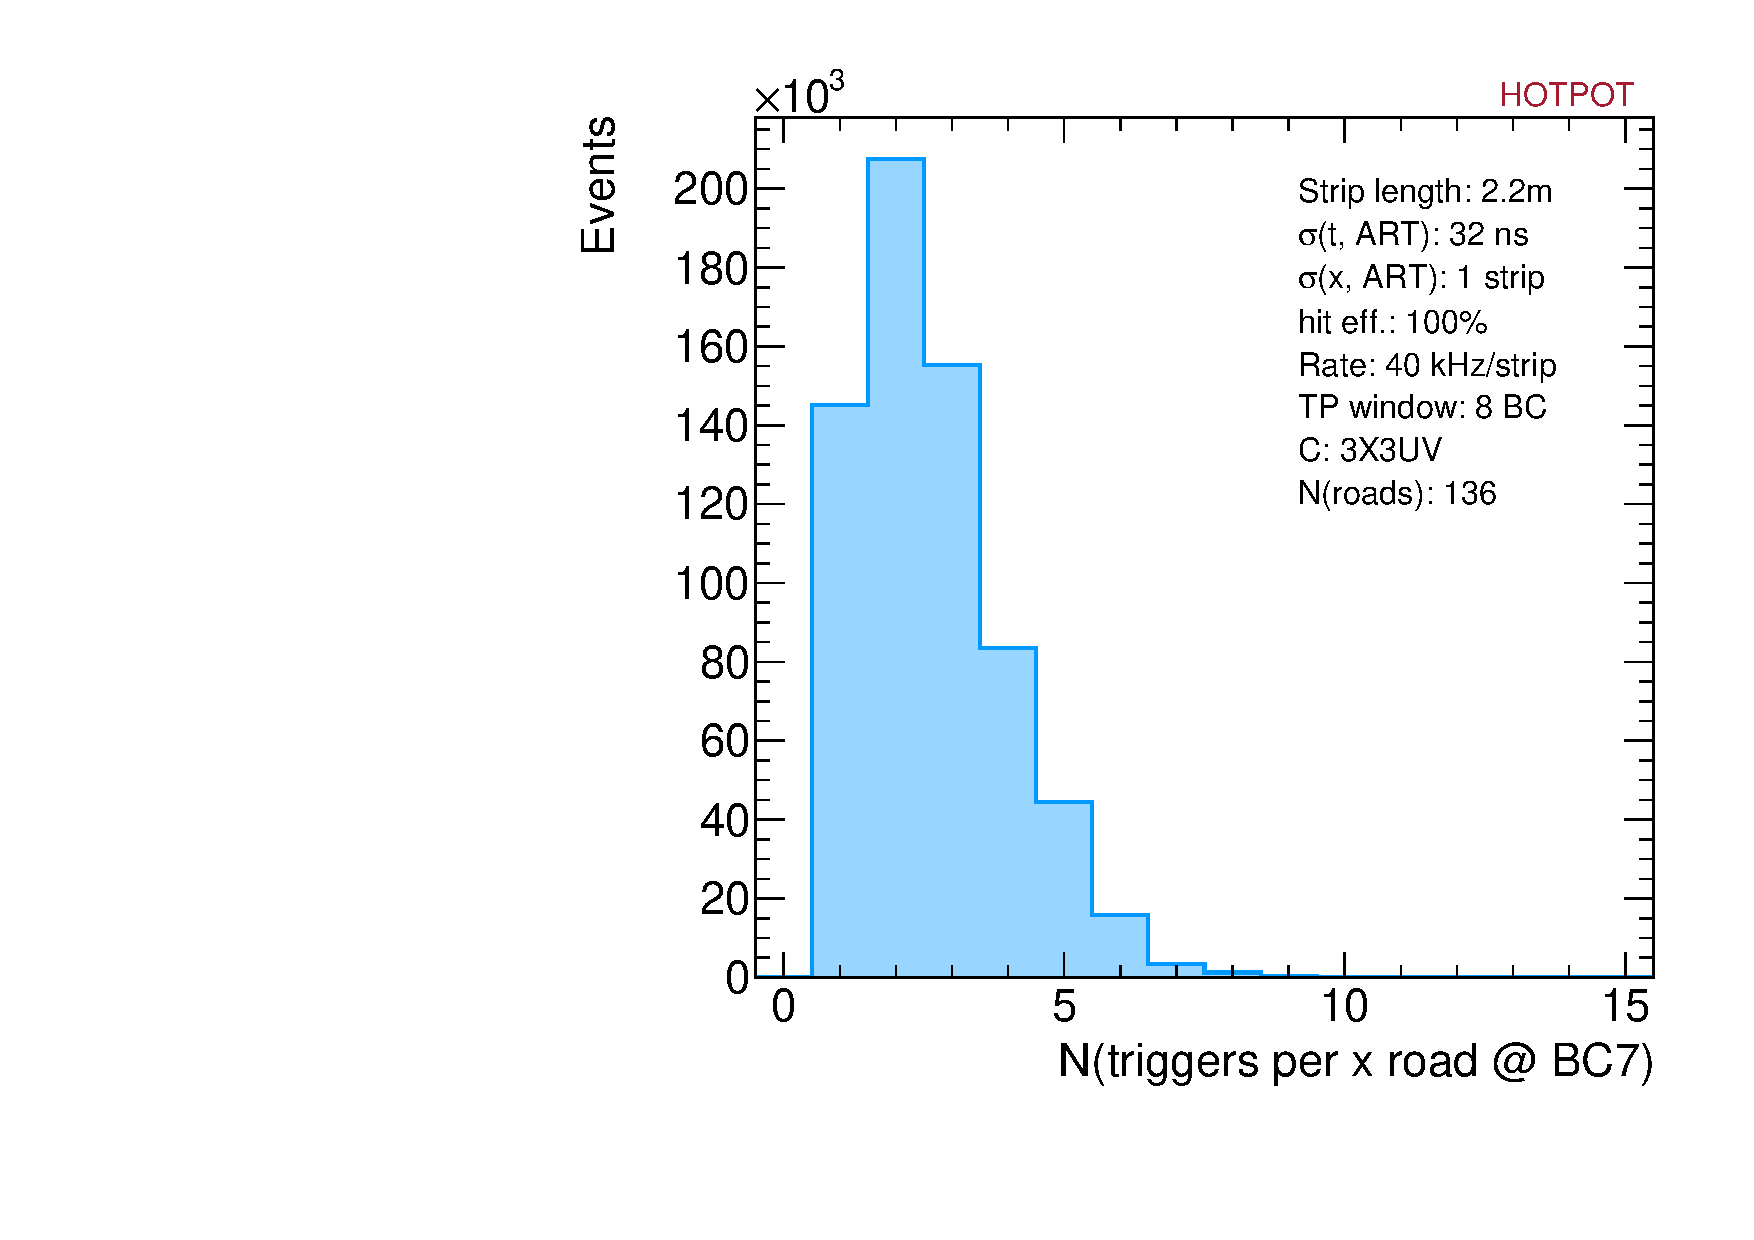
\includegraphics[width=0.48\textwidth]{figures/large_trigs_per_x.pdf}
  \end{center}
  \vspace{-10pt}
  \caption{Number of triggers found per BC associated to a given $X$ road for 0.5m long strips (left) and 2.2m long strips (right) with a 3X3UV requirement. }
  \label{fig:trig_per_x}
\end{figure}

\begin{figure}[!htpb]
  \begin{center}
    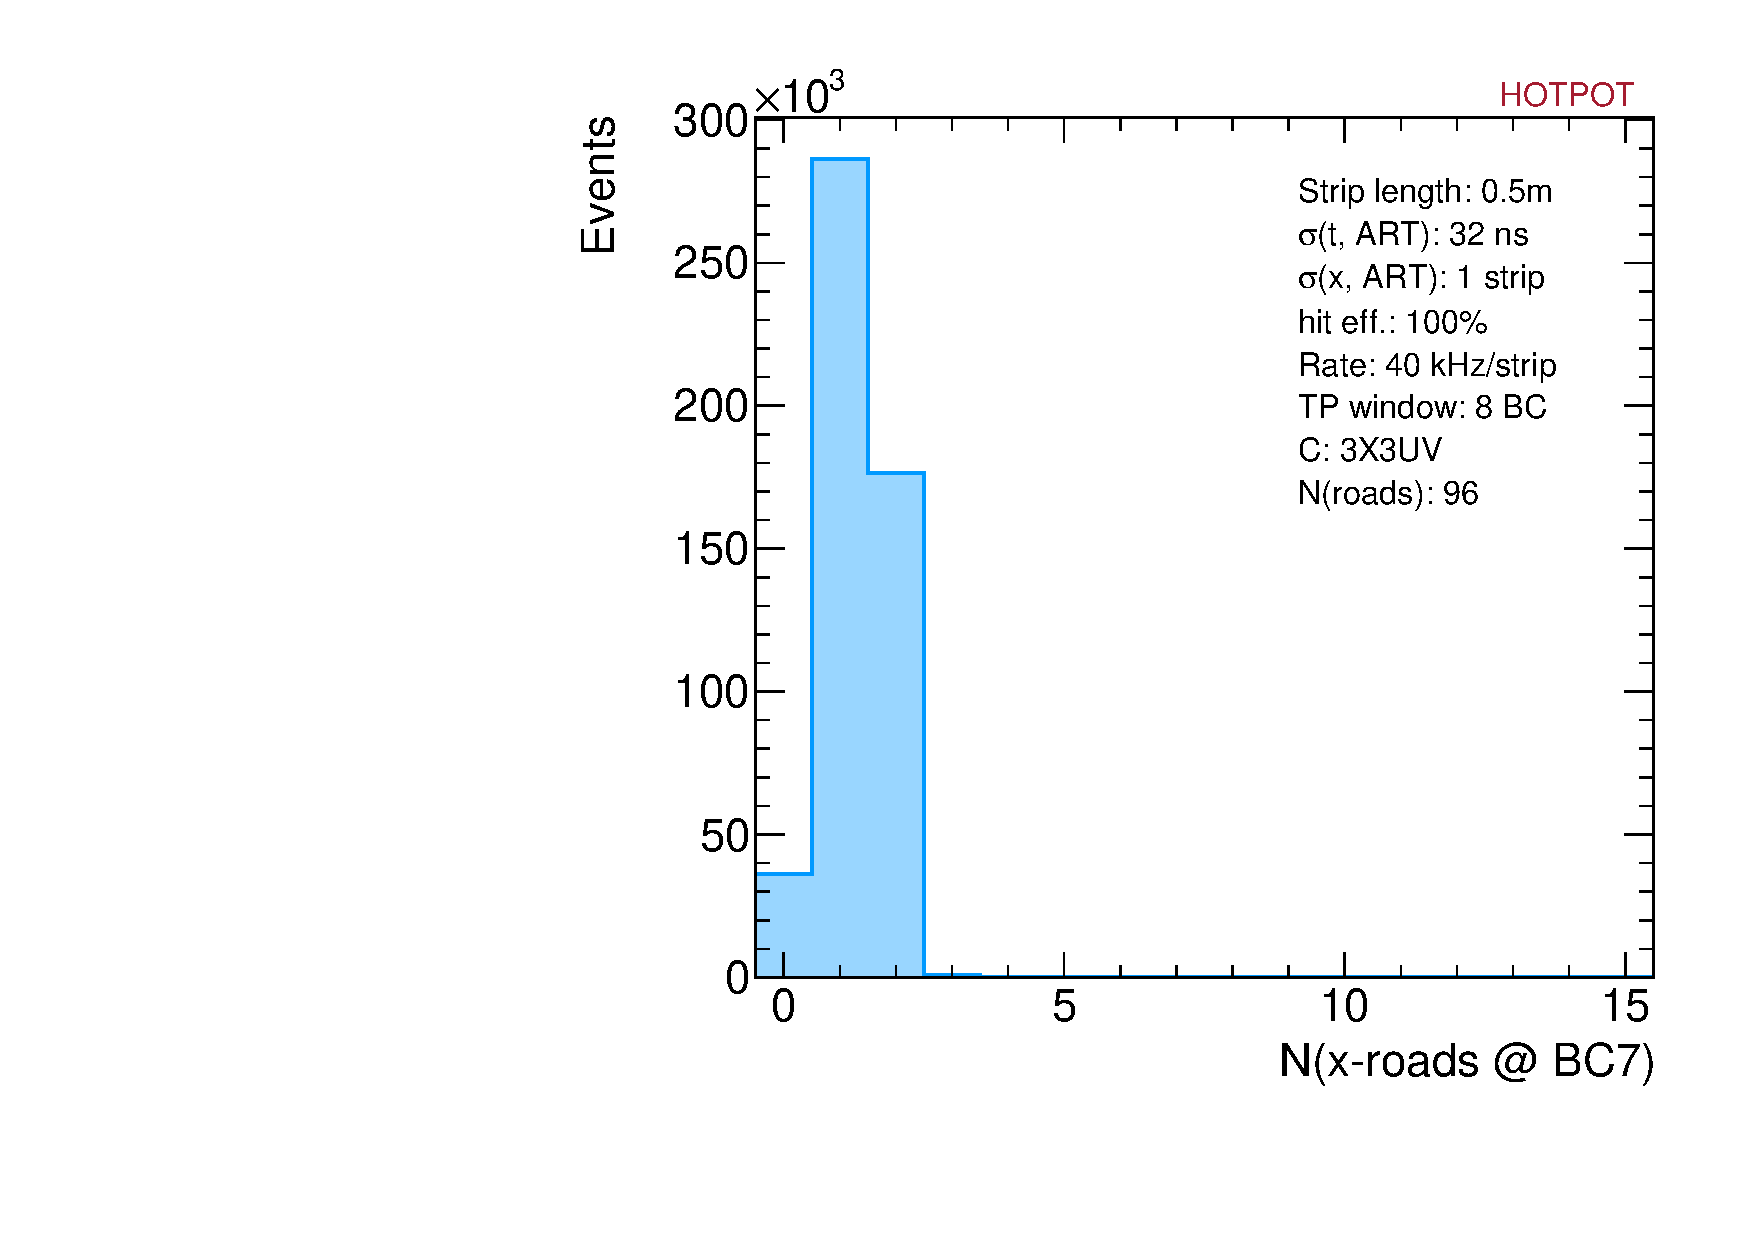
\includegraphics[width=0.48\textwidth]{figures/small_xroads.pdf}
    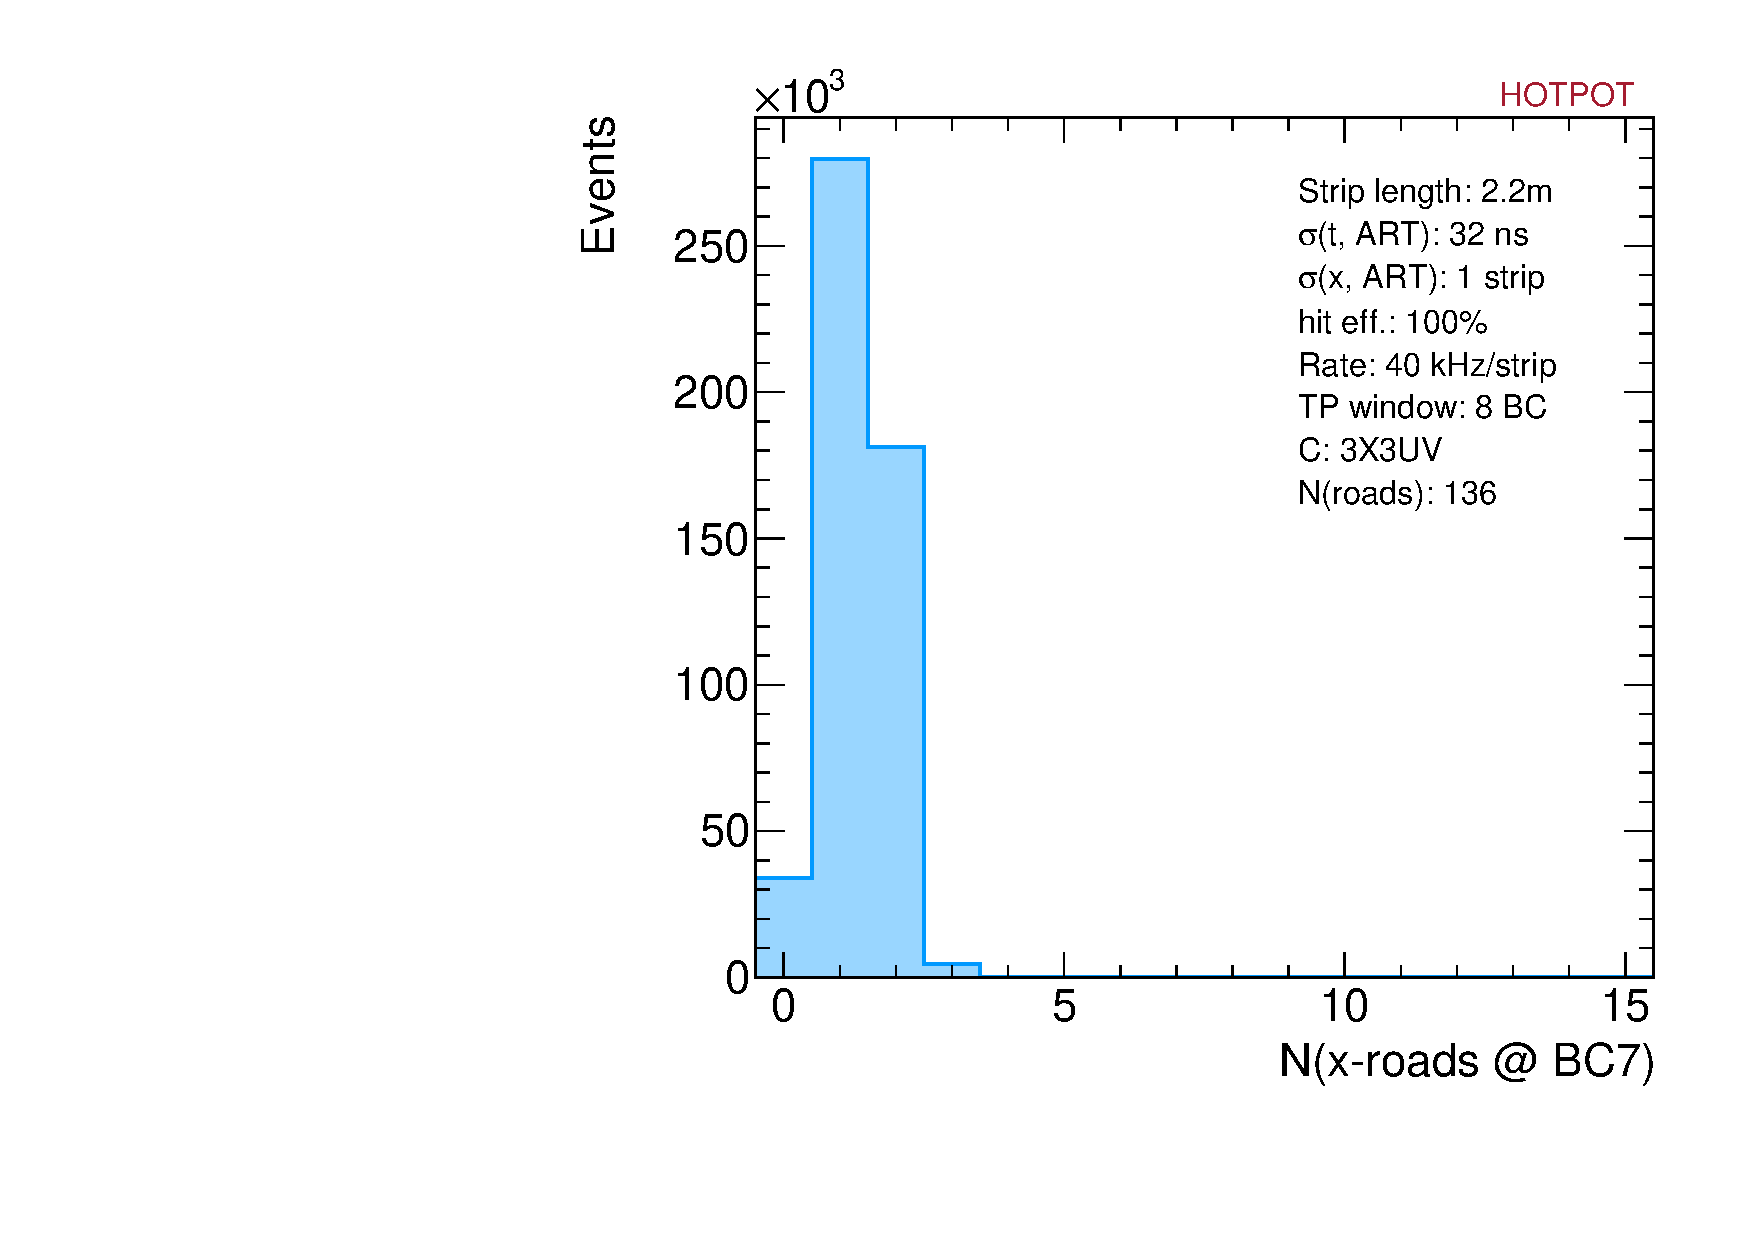
\includegraphics[width=0.48\textwidth]{figures/large_xroads.pdf}
  \end{center}
  \vspace{-10pt}
  \caption{Number of $X$ roads found per BC for 0.5m long strips (left) and 2.2m long strips (right) with a 3X3UV requirement. }
  \label{fig:xroads}
\end{figure}

Figure \ref{fig:3x_trig} shows the number of expected triggers found at the 3X stage if we assume 40 kHz of uncorrelated background. Again, we look at the BC in which the first real muon hit has been in the MMTP buffer for 8 BCs. The distribution, when there is a real muon track, has a tail up to 5 $X$ roads triggering in a given BC. Figure \ref{fig:trig_per_x} shows the distribution of 3X3UV triggers associated to a single $X$ road, which can be as many as 9-10. However, if we look at the number of unique $X$ roads associated to the 3X3UV triggers, shown in Fig. \ref{fig:xroads}, we see that the distribution peaks at a smaller value than the number of 3X triggers, shown in Fig. \ref{fig:3x_trig}. This indicates that a significant portion of the $X$ roads which pass the stage I pre-filter do not form stage II triggers.
\begin{figure}[!htpb]
  \begin{center}
    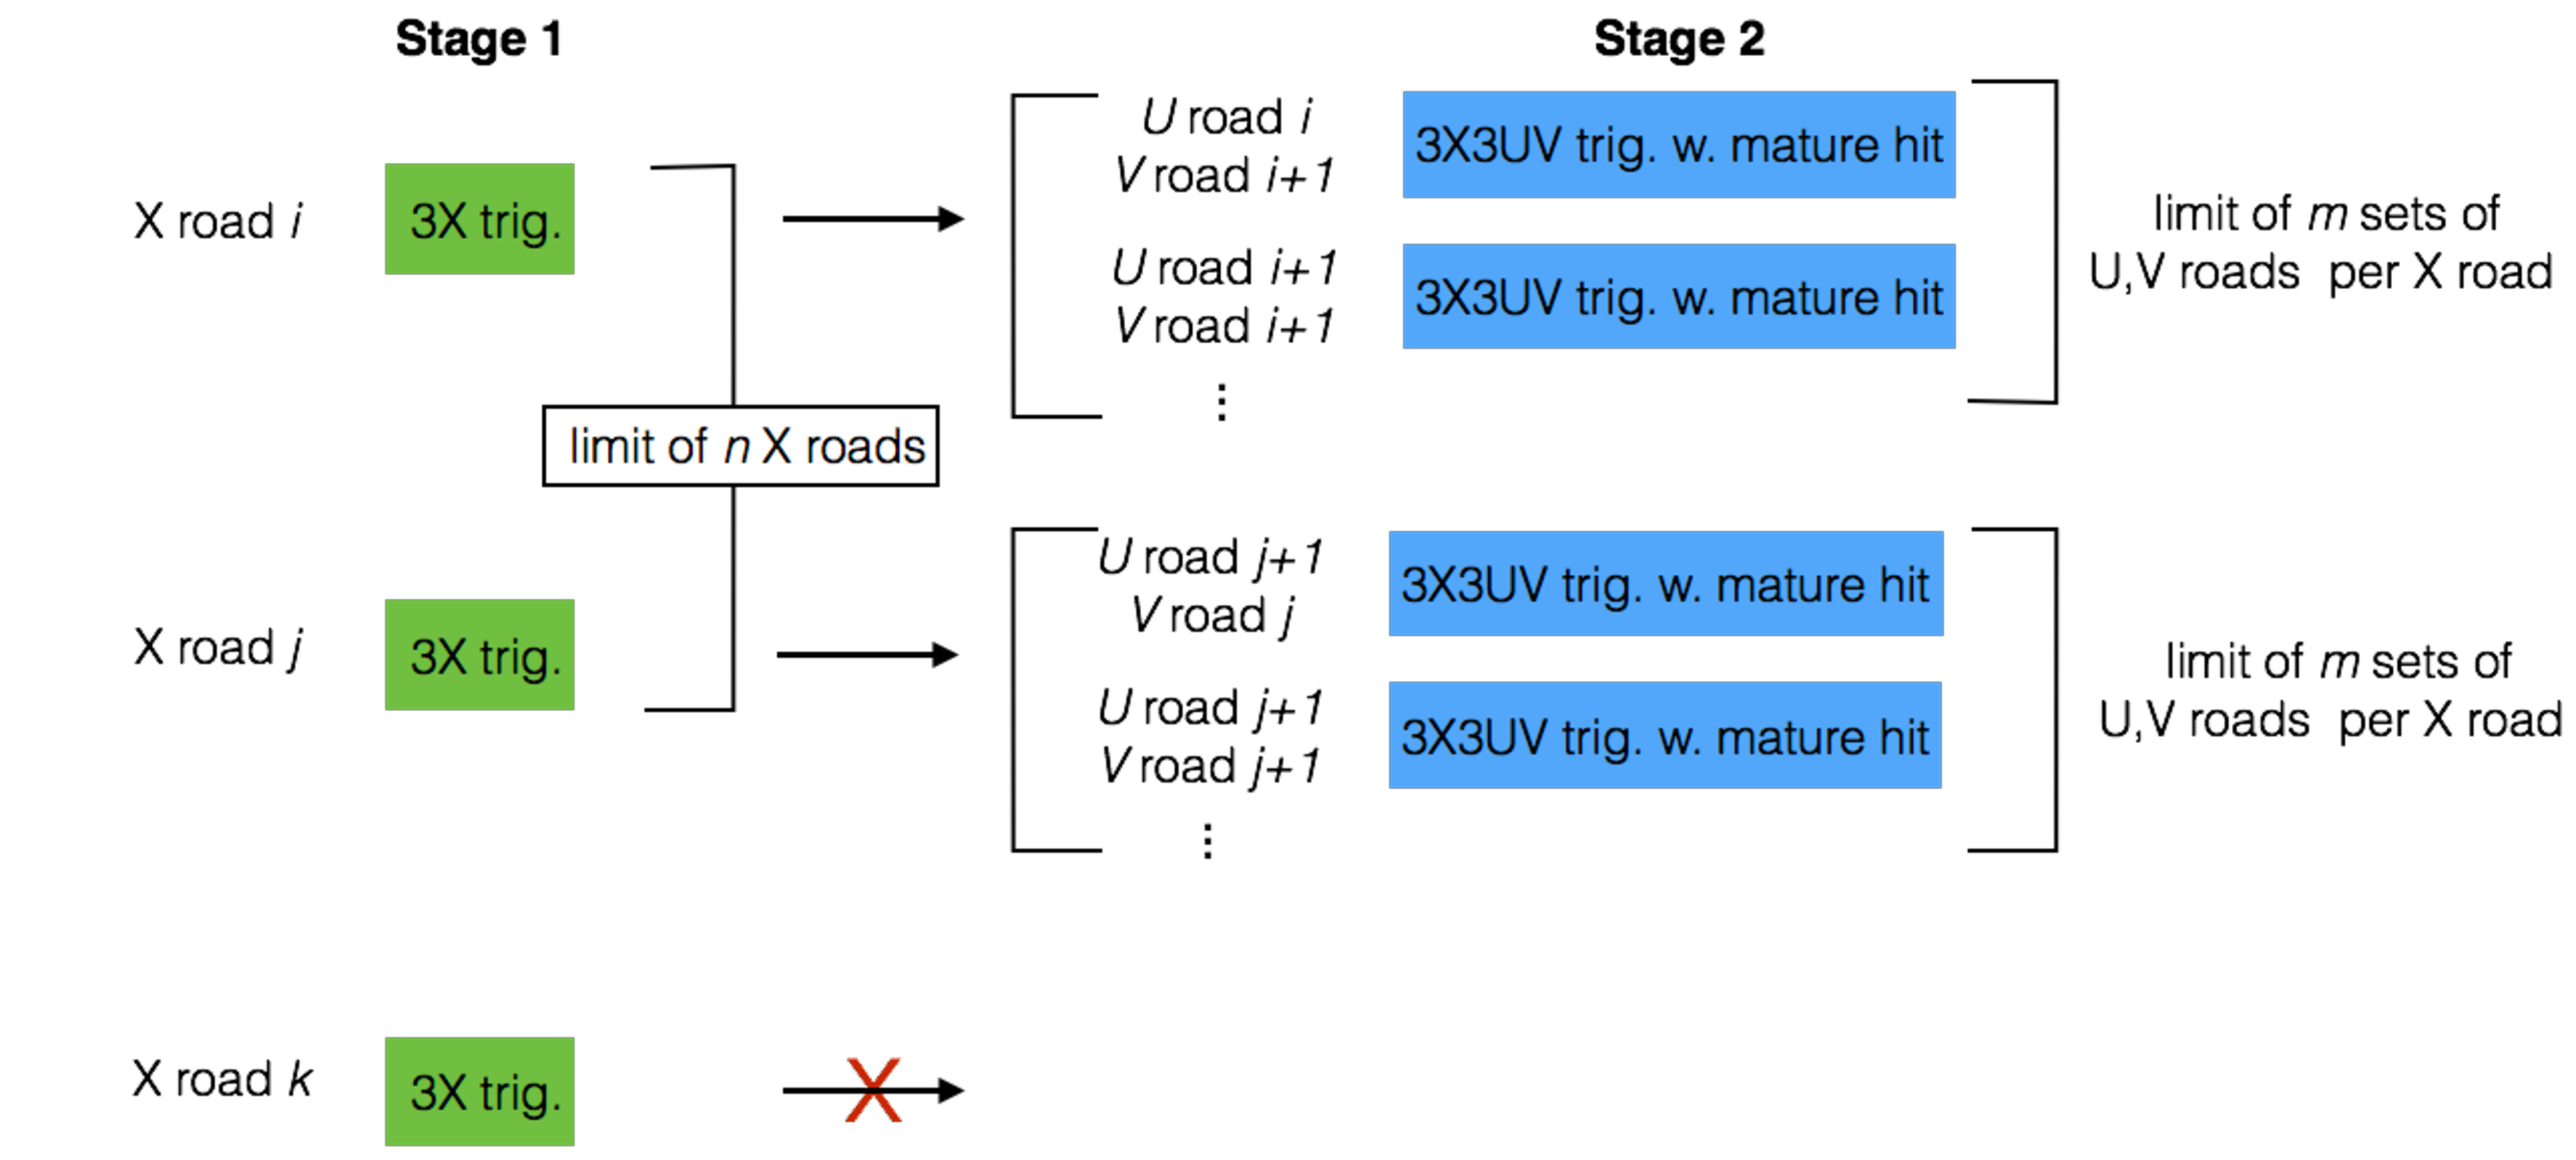
\includegraphics[width=0.96\textwidth]{figures/multistage.pdf}
  \end{center}
  \vspace{-10pt}
  \caption{Schematic of the two-stage filter for triggers. In stage I, up to \textit{n} X-roads with 3 x-plane hits are processed. In stage II, for each of these X-roads, the MMTP processes up to \textit{m} sets of $U$,$V$ roads. The total number $n \times m$ is currently limited to 8, set by the speed of the mother clock in the algorithm. }
  \label{fig:mstage}
\end{figure}

\input{tex/conclusion}

\clearpage

\begin{thebibliography}{99}
\label{bibliography}
\setlength{\itemsep}{1.5pt plus 2.0pt minus 1.4pt}
\setlength{\parsep}{0pt}
\setlength{\parskip}{0pt}
\vspace{-6pt}
\bibitem{nswtdr} ATLAS New Small Wheel Technical Design Report. \href{http://cds.cern.ch/record/1552862}{\color{blue}\underline{ATLAS-TDR-020}}.
 \href{https://cds.cern.ch/record/2272355}{\color{blue}\underline{ATL-COM-MUON-2017-036}}.
\bibitem{noisy} P.~Giromini {\it et al,} Performance of a Micromegas octuplet in the time  of noise.
 \href{https://cds.cern.ch/record/2277316}{\color{blue}\underline{ATL-COM-MUON-2017-036}}.
\bibitem{noiseless} P.~Giromini  {\it et al,} Performance of a Micromegas octuplet after removing the major cause of noise.
 \href{https://cds.cern.ch/record/2277316}{\color{blue}\underline{ATL-COM-MUON-2017-040}}.
\bibitem{mmfe8} \url{https://twiki.cern.ch/twiki/bin/viewauth/Atlas/NewSmallWheel}.
\bibitem{addc} \url{https://twiki.cern.ch/twiki/pub/Atlas/February_2015_design_reviews/ADDC_document_for_2015_Feb_NSW_review_v1.0.pdf}.
\bibitem{brian} B.~Clark {\it et al,} An Algorithm for Micromegas Segment
 Reconstruction in the Level-1 Trigger of the New Small Wheel. \href{https://cds.cern.ch/record/1706160}{\color{blue}\underline{ATL-COM-UPGRADE-2014-012}}.
\bibitem{steve} S.~Chan et. al. Micromegas Trigger Processor Algorithm Performance in Nominal, Misaligned, and Misalignment
 Corrected Conditions. \href{https://cds.cern.ch/record/2113121}{\color{blue}\underline{ATL-COM-UPGRADE-2015-033}}.
\bibitem{oldart} K.~DiPetrillo  {it et al,} ATL-COM-MUON-2014-069.
\bibitem{koki} Simulation of the ATLAS New Small Wheel (NSW) System
 \href{http://cds.cern.ch/record/2265067}{\color{blue}\underline{ATL-MUON-SLIDE-2017-248}}.
\bibitem{phase2} ATLAS Muon Spectrometer Phase-II Upgrade Technical Design Report.
 \href{https://cds.cern.ch/record/2270169/}{\color{blue}\underline{ATL-COM-MUON-2017-033}}.
\bibitem{mmtp} J. ~Farah {\it et al,} Test of the Micromegas Trigger Processor with Cosmic Ray Muons. 
\href{https://cds.cern.ch/record/2285496}{\color{blue}\underline{ATL-COM-MUON-2017-049}}.
\bibitem{lhc} LHC Design Report. 
 \href{https://cds.cern.ch/record/782076}{\color{blue}\underline{CERN-2004-003}}.
\bibitem{tuna} A. N. Tuna. Studies of the ATLAS MDT and CSC hit rates using proton-proton collisions at 13 TeV. 
  \href{https://cds.cern.ch/record/2111365}{\color{blue}\underline{ATL-COM-MUON-2015-098}}.
\end{thebibliography}










\end{document} 

